\documentclass[13pt,a4paper]{report}
\usepackage[margin=0.6in]{geometry}
\usepackage{fancybox}
\usepackage[utf8]{inputenc}
\usepackage[vietnamese,main=english]{babel}
\usepackage{multicol}
\usepackage{tabularx}
\usepackage{lmodern}
\usepackage{minted}
\usepackage{indentfirst}
\usepackage{float}
\usepackage{enumitem}
\usepackage{afterpage}
\usepackage[super]{nth}
\usepackage{titlesec}
\usepackage{bigdelim}
\usepackage[titles]{tocloft}
\usepackage{makecell}
\usepackage{arydshln}
\usepackage{perpage} %the perpage package
\usepackage{graphicx}
\usepackage{caption}
\usepackage{gensymb}
\usepackage{tikz}
\usepackage{circuitikz}
\usepackage{pgfplots}
\usepackage{cancel}
\usepackage{xurl}
\usepackage[bottom]{footmisc}
\usepackage[font=footnotesize,labelfont={scriptsize}]{subfig}
\usepackage{wrapfig}
\usepackage{latexsym,amssymb,amsmath}
%\usepackage{algpseudocode}
\usepackage{tocvsec2}
\usepackage{fancyref}
\usepackage{bookmark}
\usepackage{hyperref}
\usepackage[nameinlink,noabbrev]{cleveref}

\newcolumntype{Y}{>{\centering\arraybackslash}X}

\PassOptionsToPackage{hyphens}{url}

\makeatletter
\pgfcircdeclarebipole{}{\ctikzvalof{bipoles/vsourceam/height}}{vsourceAM}{\ctikzvalof{bipoles/vsourceam/height}}{\ctikzvalof{bipoles/vsourceam/width}}{%
  \pgfsetlinewidth{\pgfkeysvalueof{/tikz/circuitikz/bipoles/thickness}\pgfstartlinewidth}
   \pgfpathellipse{\pgfpointorigin}{\pgfpoint{0}{\pgf@circ@res@up}}{\pgfpoint{\pgf@circ@res@left}{0}}
   \pgfusepath{draw}
   \pgfscope
       \pgftransformxshift{0.6*\ctikzvalof{bipoles/vsourceam/margin}\pgf@circ@res@left}
       \pgftext[rotate=-\pgf@circ@direction]{$+$}
       \pgfusepath{draw}
   \endpgfscope
   \pgfscope
       \pgftransformxshift{0.6*\ctikzvalof{bipoles/vsourceam/margin}\pgf@circ@res@right}
       \pgftext[rotate=-\pgf@circ@direction]{$-$}
       \pgfusepath{draw}
   \endpgfscope
}
\makeatother

\MakePerPage{footnote} %the perpage package command
\usetikzlibrary{shapes,positioning,arrows,calc}

\newcommand*\justify{%
  \fontdimen2\font=0.4em% interword space
  \fontdimen3\font=0.2em% interword stretch
  \fontdimen4\font=0.1em% interword shrink
  \fontdimen7\font=0.1em% extra space
  \hyphenchar\font=`\-% allowing hyphenation
}
\renewcommand\cftchapafterpnum{\vskip-2pt}
\renewcommand\cftsecafterpnum{\vskip-2pt}

\renewcommand{\theequation}{\arabic{equation}}

% FLOW CHART
\tikzstyle{startstop} = [rectangle, rounded corners, minimum width=3cm, minimum height=1cm,text centered, draw=black, fill=red!30]
\tikzstyle{io} = [trapezium, trapezium left angle=70, trapezium right angle=110, minimum width=3cm, minimum height=1cm, text centered, draw=black, fill=blue!30]
\tikzstyle{process} = [rectangle, minimum width=3cm, minimum height=1cm, text centered, draw=black, fill=orange!30, text width=4cm]
\tikzstyle{decision} = [diamond, aspect=2.5, minimum width=3cm, minimum height=1cm, text centered, draw=black, fill=green!30]
\tikzstyle{arrow} = [thick,->,>=stealth]

% CHAPTER FORMAT
\titleformat{\chapter}%[display]
{\bfseries\fontsize{25}{30}\selectfont\raggedright}% Format and size of title text
{\llap{%
    \rule[-6pt]{6cm}{1.18cm}\rule{6pt}{0pt}}% Black box to the left, lowered 6pt. The end rule is a horisontal space.
  \llap{% Number also to the left, on top of the black box.
    \fontsize{22}{44}\selectfont\color{white}\thechapter\rule{10pt}{0pt}}}{0pt}{}{}

\counterwithin{figure}{section}
\renewcommand{\thefigure}{\arabic{chapter}.\arabic{section}.\alph{figure}}

\renewcommand{\thetable}{\arabic{table}}

\renewcommand\labelitemi{$-$}
  
\titleformat{\section}
  {\LARGE\bfseries}{}{}{}
\renewcommand\thesection{\arabic{section}.}
\renewcommand\thesubsection{\arabic{subsection}}
\makeatletter
\renewcommand*\l@section{\@dottedtocline{1}{1.5cm}{2em}}
\renewcommand\section{\@startsection {section}{1}{-1em}%
  {-3.5ex \@plus -1ex \@minus -.2ex}%
  {2.3ex \@plus.2ex}%
  {\normalfont\Large\bfseries}}
\def\sectionmark#1{%
      \markright {\MakeUppercase{#1}}}
\makeatother

\titleformat{\subsection}
  {\normalfont\bfseries}{\thesubsection.}{0.5em}{}
\renewcommand\cftsubsecaftersnum{.} 
\renewcommand\thesubsection{\alph{subsection}}

\addto{\captionsenglish}{%
  \renewcommand{\bibname}{References}
}

%\addtocontents{toc}{\setcounter{tocdepth}{2}}
%\addtocontents{lof}{\vskip -1.6cm}
%\addtocontents{lot}{\vskip -1.6cm}

    
% TOC settings
\renewcommand\cftchapnumwidth{2.8em}
\renewcommand\cftsecnumwidth{3em}
\renewcommand\cftsecindent{3em}
\renewcommand\cftsubsecindent{5em}
\renewcommand\thechapter{\Roman{chapter}}
    
%\titleformat{\chapter}[display]{\normalfont\huge\bfseries}{}{0pt}{\Huge}
\newcommand{\hsp}{\hspace{20pt}}
%\titleformat{\chapter}[hang]{\Huge\bfseries}{\thechapter\hsp\textcolor{gray75}{|}\hsp}{0pt}{\Huge\bfseries}
\titleformat*{\subsubsection}{\large\bfseries}
%\titlespacing*{\chapter}{0pt}{0pt}{0pt}
    
\newcolumntype{P}[1]{>{\centering\arraybackslash}p{#1}}
\newcolumntype{C}{>{\centering\arraybackslash}p{4em}}
    
\setlist[itemize]{noitemsep, topsep=0pt}
%\AtBeginEnvironment{multicols}{\RaggedRight}

\titlespacing*{\chapter}{0pt}{0pt}{20pt}

\newcommand\Chapter[2]{\chapter
  [#1\text{: }\hfil\hbox{}\protect\linebreak{\itshape#2}]%
  {#1\\[-0.75ex]\Large#2}%
  \markboth{\MakeUppercase{\chaptername\ \thechapter.\ #1}}{}%
}


\def\doubleoverline#1{\overline{\overline{#1}}}

\captionsetup[subfloat]{labelformat=empty}

\begin{document}
%Trang bìa 1
\fontsize{13pt}{18pt}\selectfont
\begin{titlepage}
\thispagestyle{empty}
\thisfancypage{%đóng khung trang này
\setlength{\fboxsep}{0pt}% 8pt là độ dày của đường viền
\fbox}{} % phần nội dung sau là tương tự như đã làm
\

\begin{center}
\begin{large}
HO CHI MINH CITY UNIVERSITY OF TECHNOLOGY $-$ VNU HCMC
\end{large} \\
\begin{large}
OFFICE FOR INTERNATIONAL STUDY PROGRAM
\end{large} \\
\begin{large}
FACULTY OF ELECTRICAL AND ELECTRONIC ENGINEERING
\end{large} \\
\textbf{--------------------  *  --------------------}\\[4cm]
\includegraphics[scale=0.1]{logobk.png}\\[1cm]
{\fontsize{20pt}{1}\selectfont DIGITAL SYSTEMS (LAB)}\\
{\fontsize{20pt}{1}\selectfont EXPERIMENTAL REPORT (Lab 3)}\\[2.5cm]
\end{center}

\begin{otherlanguage}{vietnamese}
\begin{tabbing}
	\hspace{3.5cm}Lecturer  \ \ \ \ \=: \textbf{\parbox[t]{9cm}{Mr. Nguyễn Tuấn Hùng}}\\
	\hspace{3.5cm}Subject \>: \textbf{\parbox[t]{12cm}{Digital Systems}}\\
	\hspace{3.5cm}Class \>: \textbf{\parbox[t]{9cm}{TT06}}\\
	\hspace{3.5cm}Name \>: \textbf{\parbox[t]{9cm}{
		Lương Triển Thắng}}\\
	\hspace{3.5cm}Student ID \>: \textbf{\parbox[t]{9cm}{
		2051194}}\\[40pt]
\end{tabbing}
\end{otherlanguage}

\vspace{2.25cm}
\begin{center}
{\fontsize{13pt}{1}\selectfont Ho Chi Minh City, \nth{7} June, 2022}
\end{center}
\end{titlepage}

\tableofcontents

\setminted{fontsize=\normalsize}

\setcounter{chapter}{2}

\Chapter{Laboratory 3}{Adders, subtractors and multipliers}

\section{Known how to program a system to add the value of an input A to itself repeatedly}
\ctikzset{logic ports=ieee}

\subsection{Code}
\subsubsection{DFFn.vhd}
\begin{minted}{vhdl}
LIBRARY ieee;
USE ieee.std_logic_1164.ALL;
ENTITY DFFn IS
	PORT (
		Din, DClk, Drst : IN STD_LOGIC;
		DQ : OUT STD_LOGIC);
END DFFn;
ARCHITECTURE Behavior OF DFFn IS
BEGIN
	PROCESS (Drst, DClk)
	BEGIN
		IF rising_edge(DClk) THEN
			DQ <= Din;
		END IF;
		IF Drst = '1' THEN
			DQ <= '0';
		END IF;
	END PROCESS;
END Behavior;
\end{minted}

\subsubsection{EightBitReg.vhd}
\begin{minted}{vhdl}
LIBRARY ieee;
USE ieee.std_logic_1164.ALL;
USE ieee.numeric_std.ALL;

ENTITY EightBitReg IS
	PORT (
		EBRClk, EBRrst : IN STD_LOGIC;
		EBRD : IN STD_LOGIC_VECTOR(7 DOWNTO 0);
		EBRQ : OUT STD_LOGIC_VECTOR(7 DOWNTO 0)
	);
END EightBitReg;

ARCHITECTURE arch OF EightBitReg IS
	COMPONENT DFFn IS
		PORT (
			Din, DClk, Drst : IN STD_LOGIC;
			DQ : OUT STD_LOGIC);
	END COMPONENT;
BEGIN
	gen : FOR i IN 7 DOWNTO 0 GENERATE
		DFFs : DFFn PORT MAP(Din => EBRD(i), DClk => EBRClk, Drst => EBRrst, DQ => EBRQ(i));
	END GENERATE;
END ARCHITECTURE;
\end{minted}

\subsubsection{HEXDisplay.vhd}
\begin{minted}{vhdl}
LIBRARY ieee;
USE ieee.std_logic_1164.ALL;

ENTITY HEXDisplay IS
	PORT (
		c : IN STD_LOGIC_VECTOR(3 DOWNTO 0);
		HEXn : OUT STD_LOGIC_VECTOR(0 TO 6)
	);
END HEXDisplay;

ARCHITECTURE behavior OF HEXDisplay IS
	SIGNAL HEX : STD_LOGIC_VECTOR(0 TO 6);
BEGIN
	HEXn <= NOT(HEX);
	WITH c SELECT
		HEX <= "1111110" WHEN "0000",
		"0110000" WHEN "0001",
		"1101101" WHEN "0010",
		"1111001" WHEN "0011",
		"0110011" WHEN "0100",
		"1011011" WHEN "0101",
		"1011111" WHEN "0110",
		"1110000" WHEN "0111",
		"1111111" WHEN "1000",
		"1111011" WHEN "1001",

		"1110111" WHEN "1010",
		"0011111" WHEN "1011",
		"1001110" WHEN "1100",
		"0111101" WHEN "1101",
		"1001111" WHEN "1110",
		"1000111" WHEN "1111",
		"0000000" WHEN OTHERS;
END behavior; -- behavior
\end{minted}

\subsubsection{Exc1.vhd}
\begin{minted}{vhdl}
LIBRARY ieee;
USE ieee.std_logic_1164.ALL;
USE ieee.numeric_std.ALL;

ENTITY Exc1 IS
	PORT (
		A : IN STD_LOGIC_VECTOR(7 DOWNTO 0);
		HEX3, HEX2, HEX1, HEX0 : OUT STD_LOGIC_VECTOR(0 TO 6);
		LEDs : OUT STD_LOGIC_VECTOR(7 DOWNTO 0);
		clkN, rstN : IN STD_LOGIC;
		carry : OUT STD_LOGIC
	);
END Exc1;

ARCHITECTURE arch OF Exc1 IS
	SIGNAL rst, clk, ofl, crr : STD_LOGIC;
	SIGNAL Qa, Qb, Qc : STD_LOGIC_VECTOR(8 DOWNTO 0);
	ATTRIBUTE KEEP : BOOLEAN;
	ATTRIBUTE KEEP OF Qc : SIGNAL IS TRUE;

	COMPONENT DFFn IS
		PORT (
			Din, DClk, Drst : IN STD_LOGIC;
			DQ : OUT STD_LOGIC);
	END COMPONENT;

	COMPONENT EightBitReg IS
		PORT (
			EBRClk, EBRrst : IN STD_LOGIC;
			EBRD : IN STD_LOGIC_VECTOR(8 DOWNTO 0);
			EBRQ : OUT STD_LOGIC_VECTOR(8 DOWNTO 0)
		);
	END COMPONENT;

	COMPONENT HEXDisplay IS
		PORT (
			c : IN STD_LOGIC_VECTOR(3 DOWNTO 0);
			HEXn : OUT STD_LOGIC_VECTOR(0 TO 6)
		);
	END COMPONENT;
BEGIN
	clk <= NOT(clkN);
	rst <= NOT(rstN);

	Qb <= STD_LOGIC_VECTOR(unsigned(Qc) + unsigned(Qa));
	EBR0 : EightBitReg PORT MAP(EBRrst => rst, EBRClk => clk, EBRD => '0' & A, EBRQ => Qa);
	EBR1 : EightBitReg PORT MAP(EBRrst => rst, EBRClk => clk, EBRD => Qb, EBRQ => Qc);
	DFF0 : DFFn PORT MAP(Drst => rst, DClk => clk, Din => crr, DQ => carry);

	LEDs <= Qc(7 DOWNTO 0);
	crr <= Qb(8);
	HEX03 : HEXDisplay PORT MAP(c => A(7 DOWNTO 4), HEXn => HEX3);
	HEX02 : HEXDisplay PORT MAP(c => A(3 DOWNTO 0), HEXn => HEX2);
	HEX01 : HEXDisplay PORT MAP(c => Qc(7 DOWNTO 4), HEXn => HEX1);
	HEX00 : HEXDisplay PORT MAP(c => Qc(3 DOWNTO 0), HEXn => HEX0);
END ARCHITECTURE;
\end{minted}

\subsection{Waveform}
\begin{figure}[H]
\centering
\includegraphics[scale=0.5]{images/Exc1_waveform.png}
\end{figure}

\subsection{Result of RTL viewer}
\begin{figure}[H]
\centering
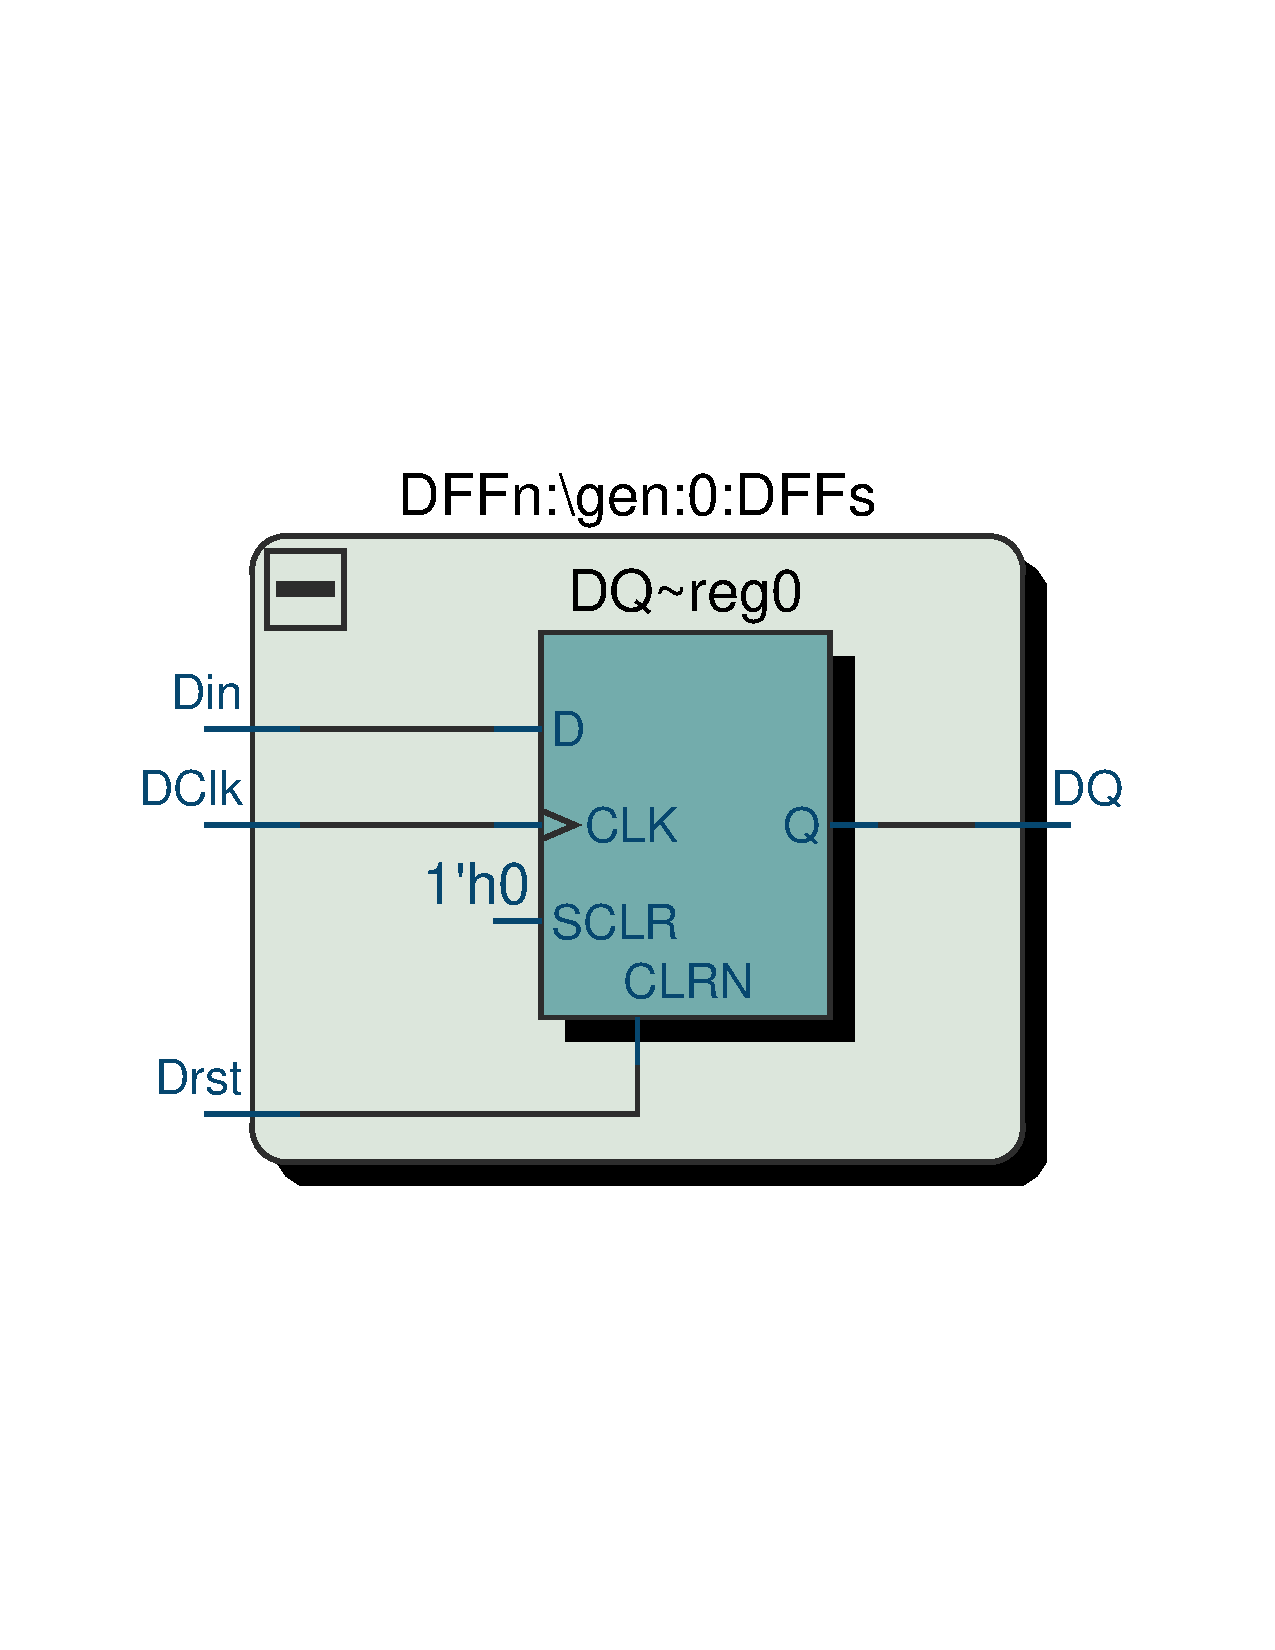
\includegraphics[scale=0.4, clip, trim={2cm 8cm 2cm 9.1cm}]{images/Exc1_DFF_RTL.pdf}
\caption*{D flip-flop}
\end{figure}

\begin{figure}[H]
\centering
\subfloat[][HEX display decoder]{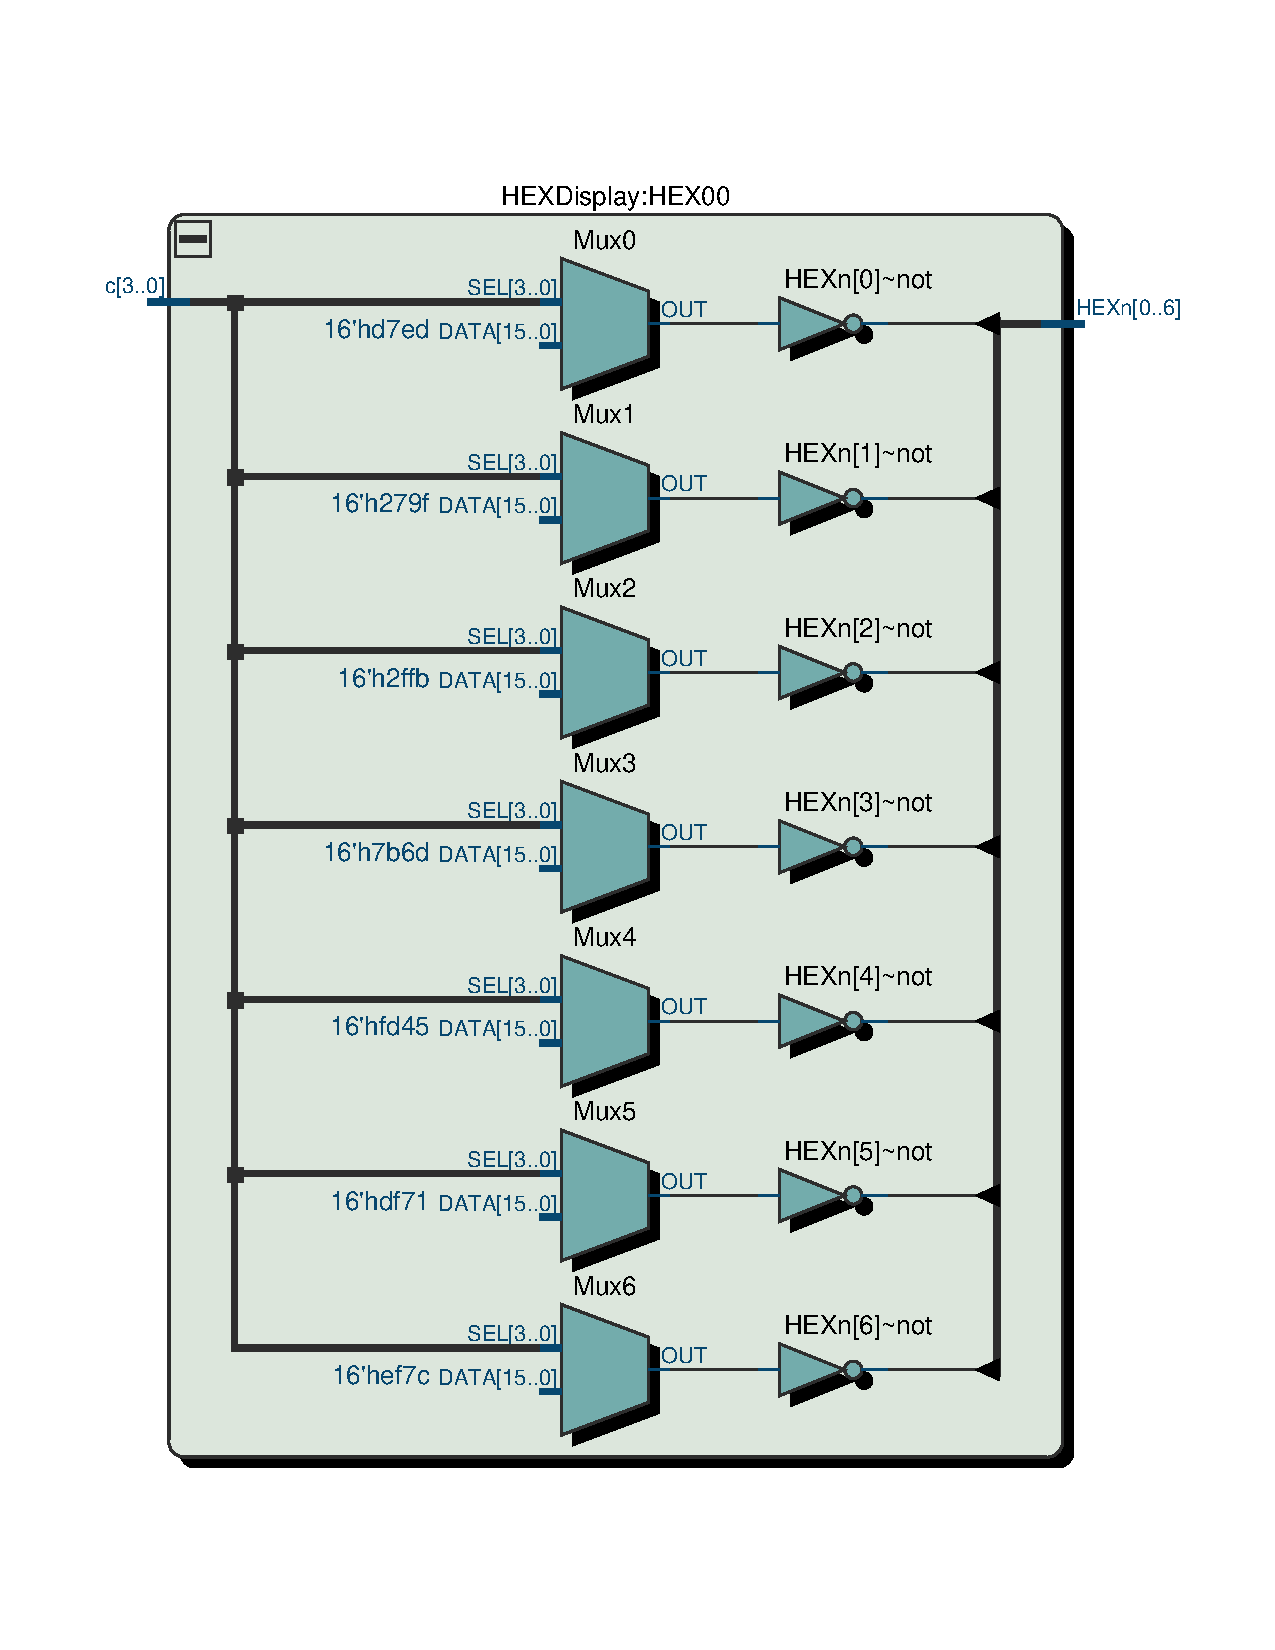
\includegraphics[scale=0.55, clip, trim={2cm 3cm 2cm 3.6cm}]{images/Exc1_HEXDisplay_RTL.pdf}}
\subfloat[][8-bit register]{\includegraphics[scale=0.45, clip, trim={3cm 1cm 3cm 1.6cm}]{images/Exc1_EightBitReg_RTL.pdf}}
\end{figure}

\begin{figure}[H]
\centering
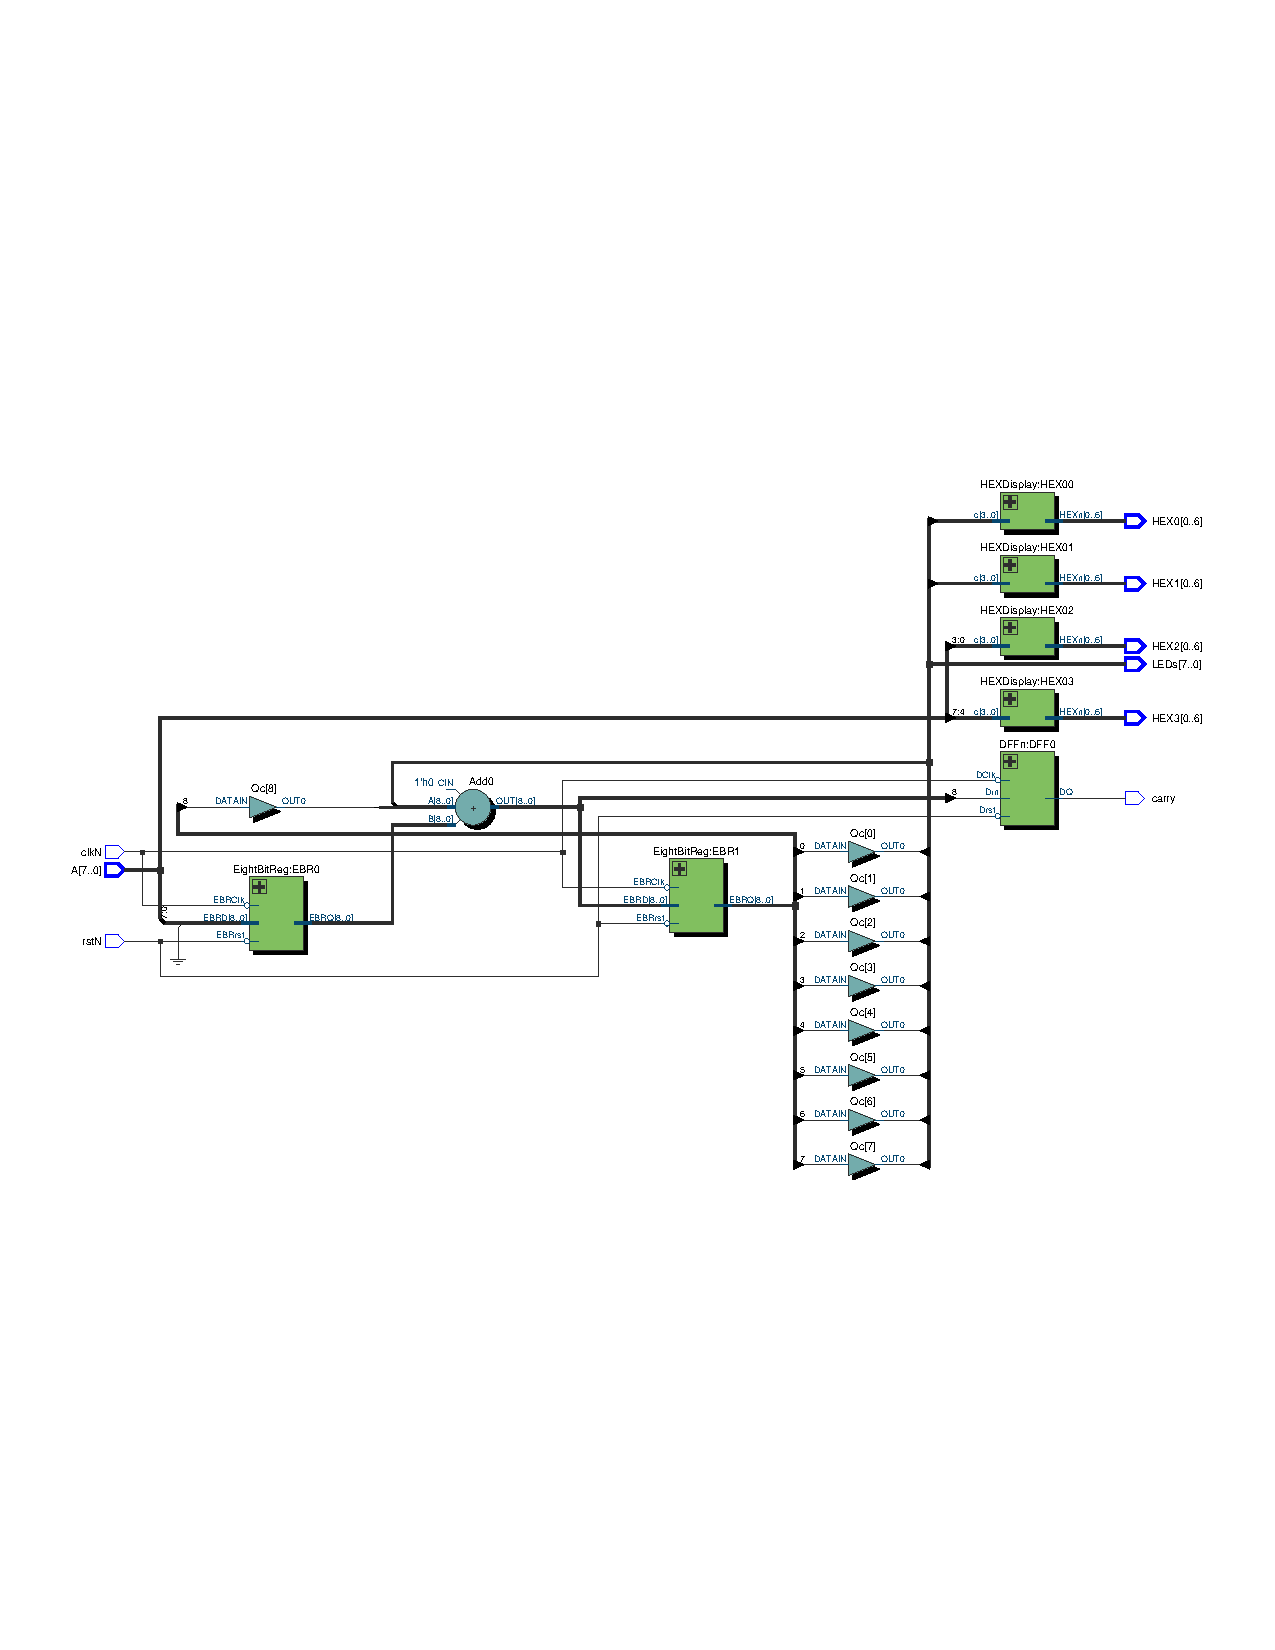
\includegraphics[scale=0.85, clip, trim={0cm 8cm 0cm 8cm}]{images/Exc1_RTL.pdf}
\caption*{Top level}
\end{figure}

\section{Known how to program a system to add or subtract the value of an input A to itself repeatedly}
\ctikzset{logic ports=ieee}

\subsection{Code}
\subsubsection{DFFn.vhd}
\begin{minted}{vhdl}
LIBRARY ieee;
USE ieee.std_logic_1164.ALL;
ENTITY DFFn IS
	PORT (
		Din, DClk, Drst : IN STD_LOGIC;
		DQ : OUT STD_LOGIC);
END DFFn;
ARCHITECTURE Behavior OF DFFn IS
BEGIN
	PROCESS (Drst, DClk)
	BEGIN
		IF rising_edge(DClk) THEN
			DQ <= Din;
		END IF;
		IF Drst = '1' THEN
			DQ <= '0';
		END IF;
	END PROCESS;
END Behavior;
\end{minted}

\subsubsection{EightBitReg.vhd}
\begin{minted}{vhdl}
LIBRARY ieee;
USE ieee.std_logic_1164.ALL;
USE ieee.numeric_std.ALL;

ENTITY EightBitReg IS
	PORT (
		EBRClk, EBRrst : IN STD_LOGIC;
		EBRD : IN STD_LOGIC_VECTOR(7 DOWNTO 0);
		EBRQ : OUT STD_LOGIC_VECTOR(7 DOWNTO 0)
	);
END EightBitReg;

ARCHITECTURE arch OF EightBitReg IS
	COMPONENT DFFn IS
		PORT (
			Din, DClk, Drst : IN STD_LOGIC;
			DQ : OUT STD_LOGIC);
	END COMPONENT;
BEGIN
	gen : FOR i IN 7 DOWNTO 0 GENERATE
		DFFs : DFFn PORT MAP(Din => EBRD(i), DClk => EBRClk, Drst => EBRrst, DQ => EBRQ(i));
	END GENERATE;
END ARCHITECTURE;
\end{minted}

\subsubsection{HEXDisplay.vhd}
\begin{minted}{vhdl}
LIBRARY ieee;
USE ieee.std_logic_1164.ALL;

ENTITY HEXDisplay IS
	PORT (
		c : IN STD_LOGIC_VECTOR(3 DOWNTO 0);
		HEXn : OUT STD_LOGIC_VECTOR(0 TO 6)
	);
END HEXDisplay;

ARCHITECTURE behavior OF HEXDisplay IS
	SIGNAL HEX : STD_LOGIC_VECTOR(0 TO 6);
BEGIN
	HEXn <= NOT(HEX);
	WITH c SELECT
		HEX <= "1111110" WHEN "0000",
		"0110000" WHEN "0001",
		"1101101" WHEN "0010",
		"1111001" WHEN "0011",
		"0110011" WHEN "0100",
		"1011011" WHEN "0101",
		"1011111" WHEN "0110",
		"1110000" WHEN "0111",
		"1111111" WHEN "1000",
		"1111011" WHEN "1001",

		"1110111" WHEN "1010",
		"0011111" WHEN "1011",
		"1001110" WHEN "1100",
		"0111101" WHEN "1101",
		"1001111" WHEN "1110",
		"1000111" WHEN "1111",
		"0000000" WHEN OTHERS;
END behavior; -- behavior
\end{minted}

\subsubsection{Exc2.vhd}
\begin{minted}{vhdl}
LIBRARY ieee;
USE ieee.std_logic_1164.ALL;
USE ieee.numeric_std.ALL;

ENTITY Exc2 IS
	PORT (
		A : IN STD_LOGIC_VECTOR(7 DOWNTO 0);
		HEX3, HEX2, HEX1, HEX0 : OUT STD_LOGIC_VECTOR(0 TO 6);
		LEDs : OUT STD_LOGIC_VECTOR(7 DOWNTO 0);
		clkN, rstN, add_sub : IN STD_LOGIC;
		carry : OUT STD_LOGIC
	);
END Exc2;

ARCHITECTURE arch OF Exc2 IS
	SIGNAL rst, clk, ofl, crr : STD_LOGIC;
	SIGNAL Qa, Qb, Qc, Qaa : STD_LOGIC_VECTOR(8 DOWNTO 0);
	ATTRIBUTE KEEP : BOOLEAN;
	ATTRIBUTE KEEP OF Qc : SIGNAL IS TRUE;
	COMPONENT DFFn IS
		PORT (
			Din, DClk, Drst : IN STD_LOGIC;
			DQ : OUT STD_LOGIC);
	END COMPONENT;

	COMPONENT EightBitReg IS
		PORT (
			EBRClk, EBRrst : IN STD_LOGIC;
			EBRD : IN STD_LOGIC_VECTOR(8 DOWNTO 0);
			EBRQ : OUT STD_LOGIC_VECTOR(8 DOWNTO 0)
		);
	END COMPONENT;

	COMPONENT BCDDisplay IS
		PORT (
			V : IN STD_LOGIC_VECTOR(7 DOWNTO 0);
			HEX02 : OUT STD_LOGIC_VECTOR(0 TO 6);
			HEX01 : OUT STD_LOGIC_VECTOR(0 TO 6);
			HEX00 : OUT STD_LOGIC_VECTOR(0 TO 6)
		);
	END COMPONENT;
	COMPONENT HEXDisplay IS
		PORT (
			c : IN STD_LOGIC_VECTOR(3 DOWNTO 0);
			HEXn : OUT STD_LOGIC_VECTOR(0 TO 6)
		);
	END COMPONENT;
BEGIN
	clk <= NOT(clkN);
	rst <= NOT(rstN);

	Qaa <= Qa WHEN add_sub = '0' ELSE STD_LOGIC_VECTOR(unsigned(NOT(Qa)) + 1);
	Qb <= STD_LOGIC_VECTOR(unsigned(Qc) + unsigned(Qaa));
	EBR0 : EightBitReg PORT MAP(EBRrst => rst, EBRClk => clk, EBRD => '0' & A, EBRQ => Qa);
	EBR1 : EightBitReg PORT MAP(EBRrst => rst, EBRClk => clk, EBRD => Qb, EBRQ => Qc);
	DFF0 : DFFn PORT MAP(Drst => rst, DClk => clk, Din => crr, DQ => carry);

	LEDs <= Qc(7 DOWNTO 0);
	crr <= Qb(8);
	HEX03 : HEXDisplay PORT MAP(c => A(7 DOWNTO 4), HEXn => HEX3);
	HEX02 : HEXDisplay PORT MAP(c => A(3 DOWNTO 0), HEXn => HEX2);
	HEX01 : HEXDisplay PORT MAP(c => Qc(7 DOWNTO 4), HEXn => HEX1);
	HEX00 : HEXDisplay PORT MAP(c => Qc(3 DOWNTO 0), HEXn => HEX0);
END ARCHITECTURE;
\end{minted}

\subsection{Waveform}
\begin{figure}[H]
\centering
\includegraphics[scale=0.5]{images/Exc2_waveform.png}
\end{figure}

\subsection{Result of RTL viewer}
\begin{figure}[H]
\centering
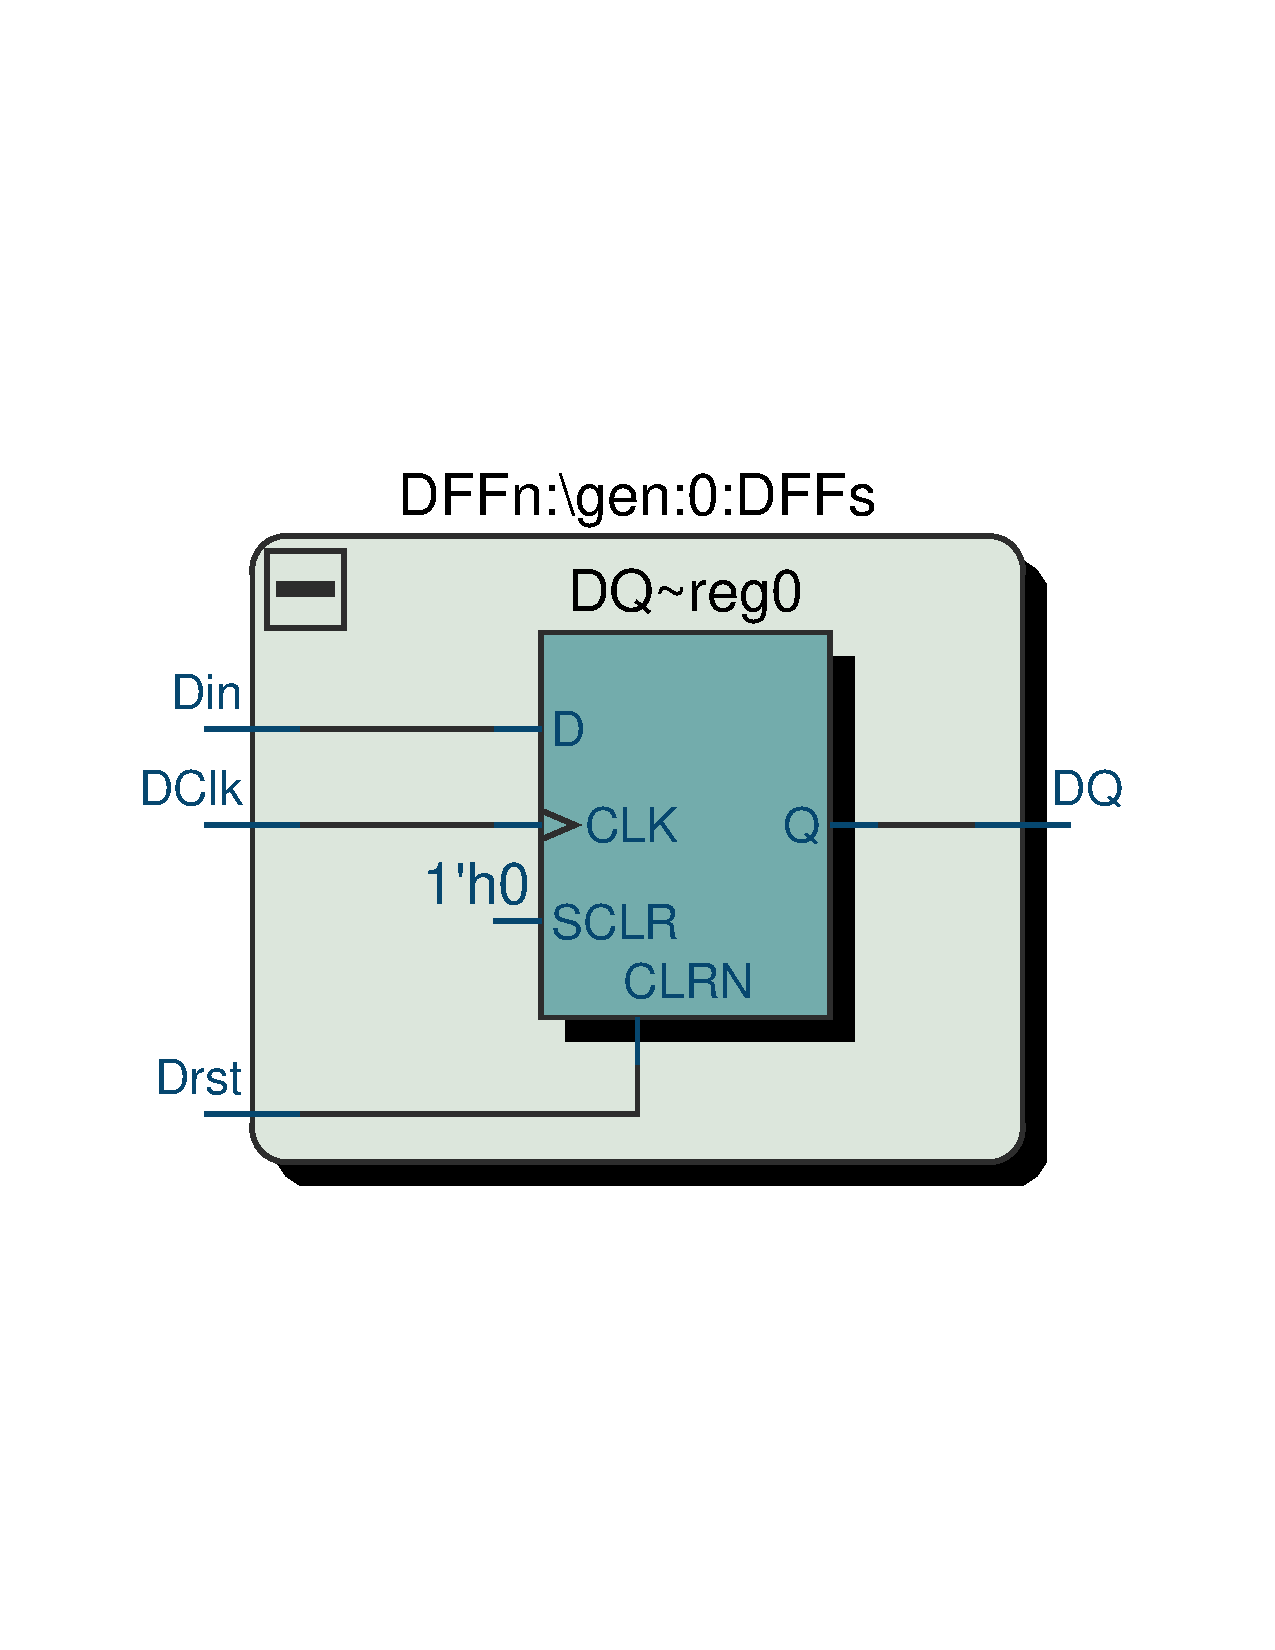
\includegraphics[scale=0.4, clip, trim={2cm 8cm 2cm 9.1cm}]{images/Exc1_DFF_RTL.pdf}
\caption*{D flip-flop}
\end{figure}

\begin{figure}[H]
\centering
\subfloat[][HEX display decoder]{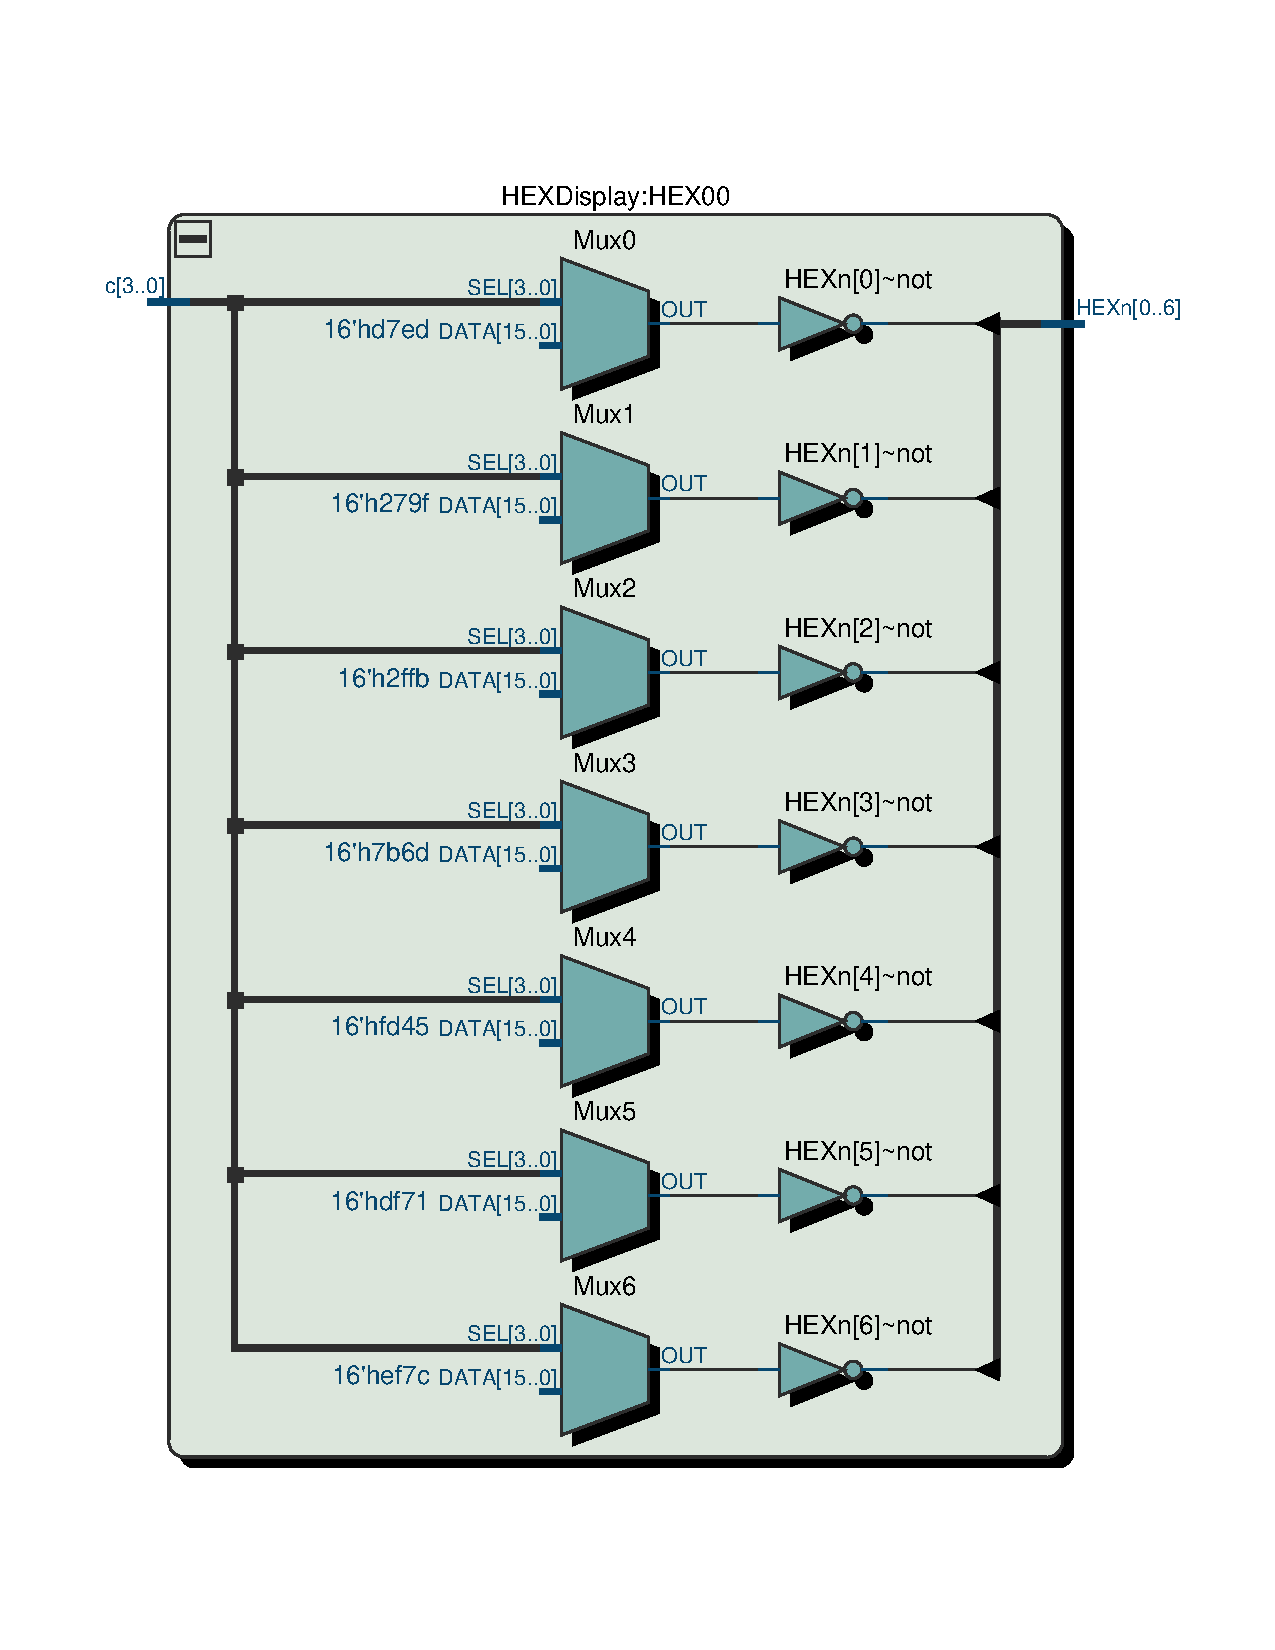
\includegraphics[scale=0.55, clip, trim={2cm 3cm 2cm 3.6cm}]{images/Exc1_HEXDisplay_RTL.pdf}}
\subfloat[][8-bit register]{\includegraphics[scale=0.45, clip, trim={3cm 1cm 3cm 1.6cm}]{images/Exc1_EightBitReg_RTL.pdf}}
\end{figure}

\begin{figure}[H]
\centering
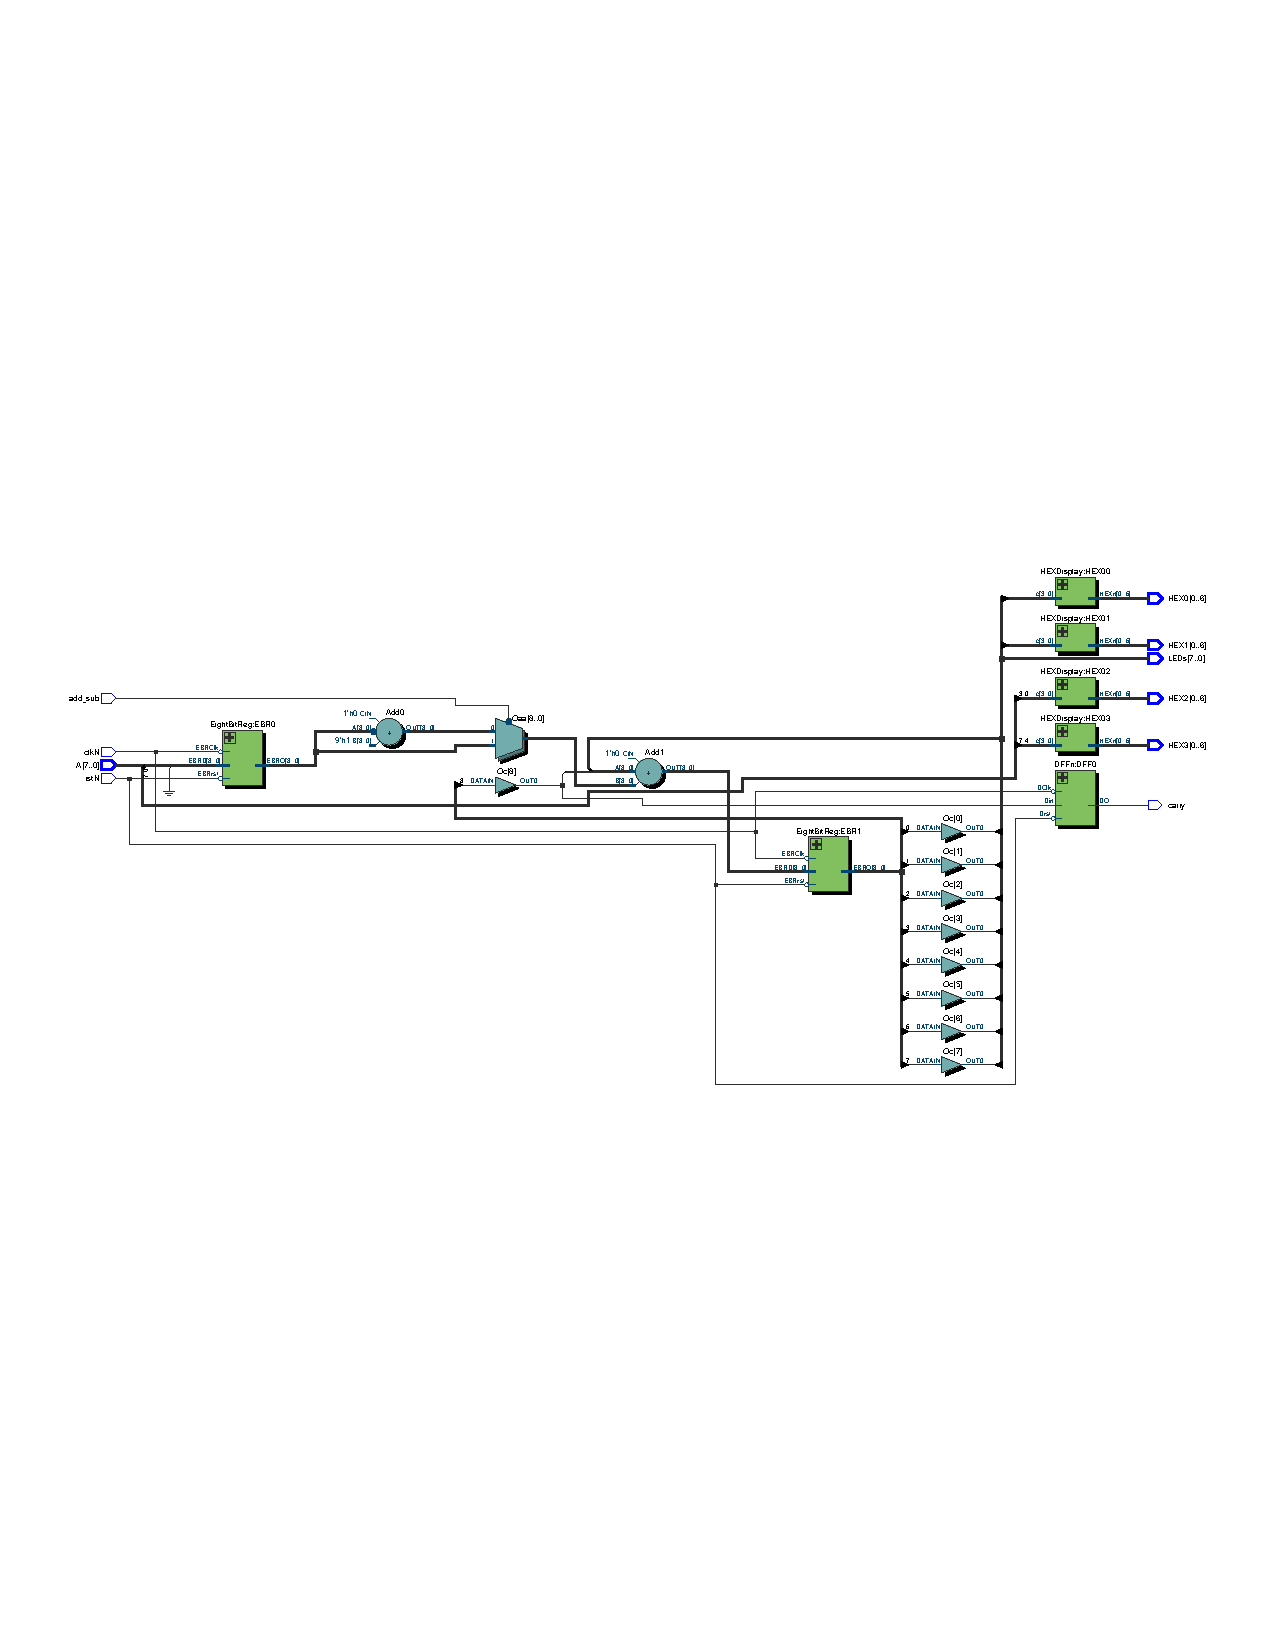
\includegraphics[scale=0.85, clip, trim={0cm 9cm 0cm 9cm}]{images/Exc2_RTL.pdf}
\caption*{Top level}
\end{figure}

\section{Known how to program 8$\times$8 multiplier circuit with registered inputs and outputs}
In this exercise, I only use two registers to store $A$ and $B$. I removed the last register so that the result can output directly without waiting for another clock.

\subsection{Code}
\subsubsection{DFFn.vhd}
\begin{minted}{vhdl}
LIBRARY ieee;
USE ieee.std_logic_1164.ALL;
ENTITY DFFn IS
	PORT (
		Din, DClk, Drst : IN STD_LOGIC;
		DQ : OUT STD_LOGIC);
END DFFn;
ARCHITECTURE Behavior OF DFFn IS
BEGIN
	PROCESS (Drst, DClk)
	BEGIN
		IF rising_edge(DClk) THEN
			DQ <= Din;
		END IF;
		IF Drst = '1' THEN
			DQ <= '0';
		END IF;
	END PROCESS;
END Behavior;
\end{minted}

\subsubsection{EightBitReg.vhd}
\begin{minted}{vhdl}
LIBRARY ieee;
USE ieee.std_logic_1164.ALL;
USE ieee.numeric_std.ALL;

ENTITY EightBitReg IS
	PORT (
		EBRClk, EBRrst : IN STD_LOGIC;
		EBRD : IN STD_LOGIC_VECTOR(7 DOWNTO 0);
		EBRQ : OUT STD_LOGIC_VECTOR(7 DOWNTO 0)
	);
END EightBitReg;

ARCHITECTURE arch OF EightBitReg IS
	COMPONENT DFFn IS
		PORT (
			Din, DClk, Drst : IN STD_LOGIC;
			DQ : OUT STD_LOGIC);
	END COMPONENT;
BEGIN
	gen : FOR i IN 7 DOWNTO 0 GENERATE
		DFFs : DFFn PORT MAP(Din => EBRD(i), DClk => EBRClk, Drst => EBRrst, DQ => EBRQ(i));
	END GENERATE;
END ARCHITECTURE;
\end{minted}

\subsubsection{Mul.vhd}
\begin{minted}{vhdl}
LIBRARY ieee;
USE ieee.std_logic_1164.ALL;
USE ieee.std_logic_unsigned.ALL;
USE IEEE.numeric_std.ALL;

ENTITY Mul IS
	PORT (
		mulA, mulB : IN STD_LOGIC_VECTOR(7 DOWNTO 0);
		mulP : OUT STD_LOGIC_VECTOR(15 DOWNTO 0)
	);
END Mul;

ARCHITECTURE arch OF Mul IS
	SIGNAL a_padded, zero : STD_LOGIC_VECTOR(15 DOWNTO 0);
	TYPE ab_t IS ARRAY(0 TO 7) OF STD_LOGIC_VECTOR(15 DOWNTO 0);
	SIGNAL ab : ab_t;
BEGIN

	zero <= "0000000000000000";
	a_padded <= "00000000" & mulA;

	ab(0) <= a_padded WHEN mulB(0) = '1' ELSE
	zero;
	sum : FOR i IN 1 TO 7 GENERATE
		ab(i) <= a_padded(15 - i DOWNTO 0) & zero(i - 1 DOWNTO 0) WHEN mulB(i) = '1' ELSE
		zero;
	END GENERATE;

	mulP <= ab(0) + ab(1) + ab(2) + ab(3) + ab(4) + ab(5) + ab(6) + ab(7);
END ARCHITECTURE;
\end{minted}

\subsubsection{HEXDisplay.vhd}
\begin{minted}{vhdl}
LIBRARY ieee;
USE ieee.std_logic_1164.ALL;

ENTITY HEXDisplay IS
	PORT (
		c : IN STD_LOGIC_VECTOR(3 DOWNTO 0);
		HEXn : OUT STD_LOGIC_VECTOR(0 TO 6)
	);
END HEXDisplay;

ARCHITECTURE behavior OF HEXDisplay IS
	SIGNAL HEX : STD_LOGIC_VECTOR(0 TO 6);
BEGIN
	HEXn <= NOT(HEX);
	WITH c SELECT
		HEX <= "1111110" WHEN "0000",
		"0110000" WHEN "0001",
		"1101101" WHEN "0010",
		"1111001" WHEN "0011",
		"0110011" WHEN "0100",
		"1011011" WHEN "0101",
		"1011111" WHEN "0110",
		"1110000" WHEN "0111",
		"1111111" WHEN "1000",
		"1111011" WHEN "1001",

		"1110111" WHEN "1010",
		"0011111" WHEN "1011",
		"1001110" WHEN "1100",
		"0111101" WHEN "1101",
		"1001111" WHEN "1110",
		"1000111" WHEN "1111",
		"0000000" WHEN OTHERS;
END behavior; -- behavior
\end{minted}

\subsubsection{Exc3.vhd}
\begin{minted}{vhdl}
LIBRARY ieee;
USE ieee.std_logic_1164.ALL;
USE ieee.numeric_std.ALL;

ENTITY Exc3 IS
	PORT (
		inp : IN STD_LOGIC_VECTOR(7 DOWNTO 0);
		HEX3, HEX2, HEX1, HEX0 : OUT STD_LOGIC_VECTOR(0 TO 6);
		enAB, clkN, rstN : IN STD_LOGIC
	);
END Exc3;

ARCHITECTURE arch OF Exc3 IS
	SIGNAL a, b : STD_LOGIC_VECTOR(7 DOWNTO 0);
	SIGNAL p : STD_LOGIC_VECTOR(15 DOWNTO 0);
	SIGNAL clk, rst : STD_LOGIC;
	COMPONENT EightBitReg IS
		PORT (
			EBRClk, EBRrst, EBRen : IN STD_LOGIC;
			EBRD : IN STD_LOGIC_VECTOR(7 DOWNTO 0);
			EBRQ : OUT STD_LOGIC_VECTOR(7 DOWNTO 0)
		);
	END COMPONENT;

	COMPONENT Mul IS
		PORT (
			mulA, mulB : IN STD_LOGIC_VECTOR(7 DOWNTO 0);
			mulP : OUT STD_LOGIC_VECTOR(15 DOWNTO 0)
		);
	END COMPONENT;

	COMPONENT HEXDisplay IS
		PORT (
			c : IN STD_LOGIC_VECTOR(3 DOWNTO 0);
			HEXn : OUT STD_LOGIC_VECTOR(0 TO 6)
		);
	END COMPONENT;
BEGIN
	rst <= NOT(rstN);
	clk <= NOT(clkN);
	EBRA : EightBitReg PORT MAP(
		EBRClk => clk, EBRrst => rst,
		EBRen => enAB, EBRD => inp, EBRQ => a);
	EBRB : EightBitReg PORT MAP(
		EBRClk => clk, EBRrst => rst,
		EBRen => NOT(enAB), EBRD => inp, EBRQ => b);

	multiplier : Mul PORT MAP(mulA => a, mulB => b, mulP => p);

	HEX03 : HEXDisplay PORT MAP(c => p(15 DOWNTO 12), HEXn => HEX3);
	HEX02 : HEXDisplay PORT MAP(c => p(11 DOWNTO 8), HEXn => HEX2);
	HEX01 : HEXDisplay PORT MAP(c => p(7 DOWNTO 4), HEXn => HEX1);
	HEX00 : HEXDisplay PORT MAP(c => p(3 DOWNTO 0), HEXn => HEX0);
END ARCHITECTURE;
\end{minted}

\newcommand{\hex}[4]{
\begin{circuitikz}
\ctikzset{seven seg/width=0.25, seven seg/thickness=3pt}
\draw (0,0) node[seven segment val=#1 dot none box off]{};
\draw (1,0) node[seven segment val=#2 dot none box off]{};
\draw (2,0) node[seven segment val=#3 dot none box off]{};
\draw (3,0) node[seven segment val=#4 dot none box off]{};
\end{circuitikz}
}
\subsection{Waveform}
% Please add the following required packages to your document preamble:
% \usepackage{multirow}
\begin{table}[H]
\centering
\begin{tabular}{cc|cccccc}
\multirow{2}{*}{$A$} & \multirow{2}{*}{$B$} & \multirow{2}{*}{$P$} & \multirow{2}{*}{7-segment display} & \multicolumn{4}{c}{HEX output (active low)} \\
                     &                      &                    &                                    & 3         & 2         & 1        & 0        \\ \hline
14                   & 83                   & 0A3C               & \hex{0}{a}{3}{c}                                   & 0000001  & 0001000   & 0000110  & 0110001  \\
8A                   & 0B                   & 05EE               &  \hex{0}{5}{e}{e}                        & 0000001   & 0100100   & 0110000 & 0110000   \\
AC                   & F3                   & A344               &  \hex{a}{3}{4}{4}                                                                   & 0001000   & 0000110  &  1001100  & 1001100   \\
81                   & CA                   & 65CA               & \hex{6}{5}{c}{a}                                   & 0100000  & 0100100  &  0110001  & 0001000 
\end{tabular}
\end{table}

\begin{figure}[H]
\centering
\includegraphics[scale=0.5]{images/Exc3_waveform.png}
\end{figure}

\subsection{Result of RTL viewer}


\begin{figure}[H]
\centering
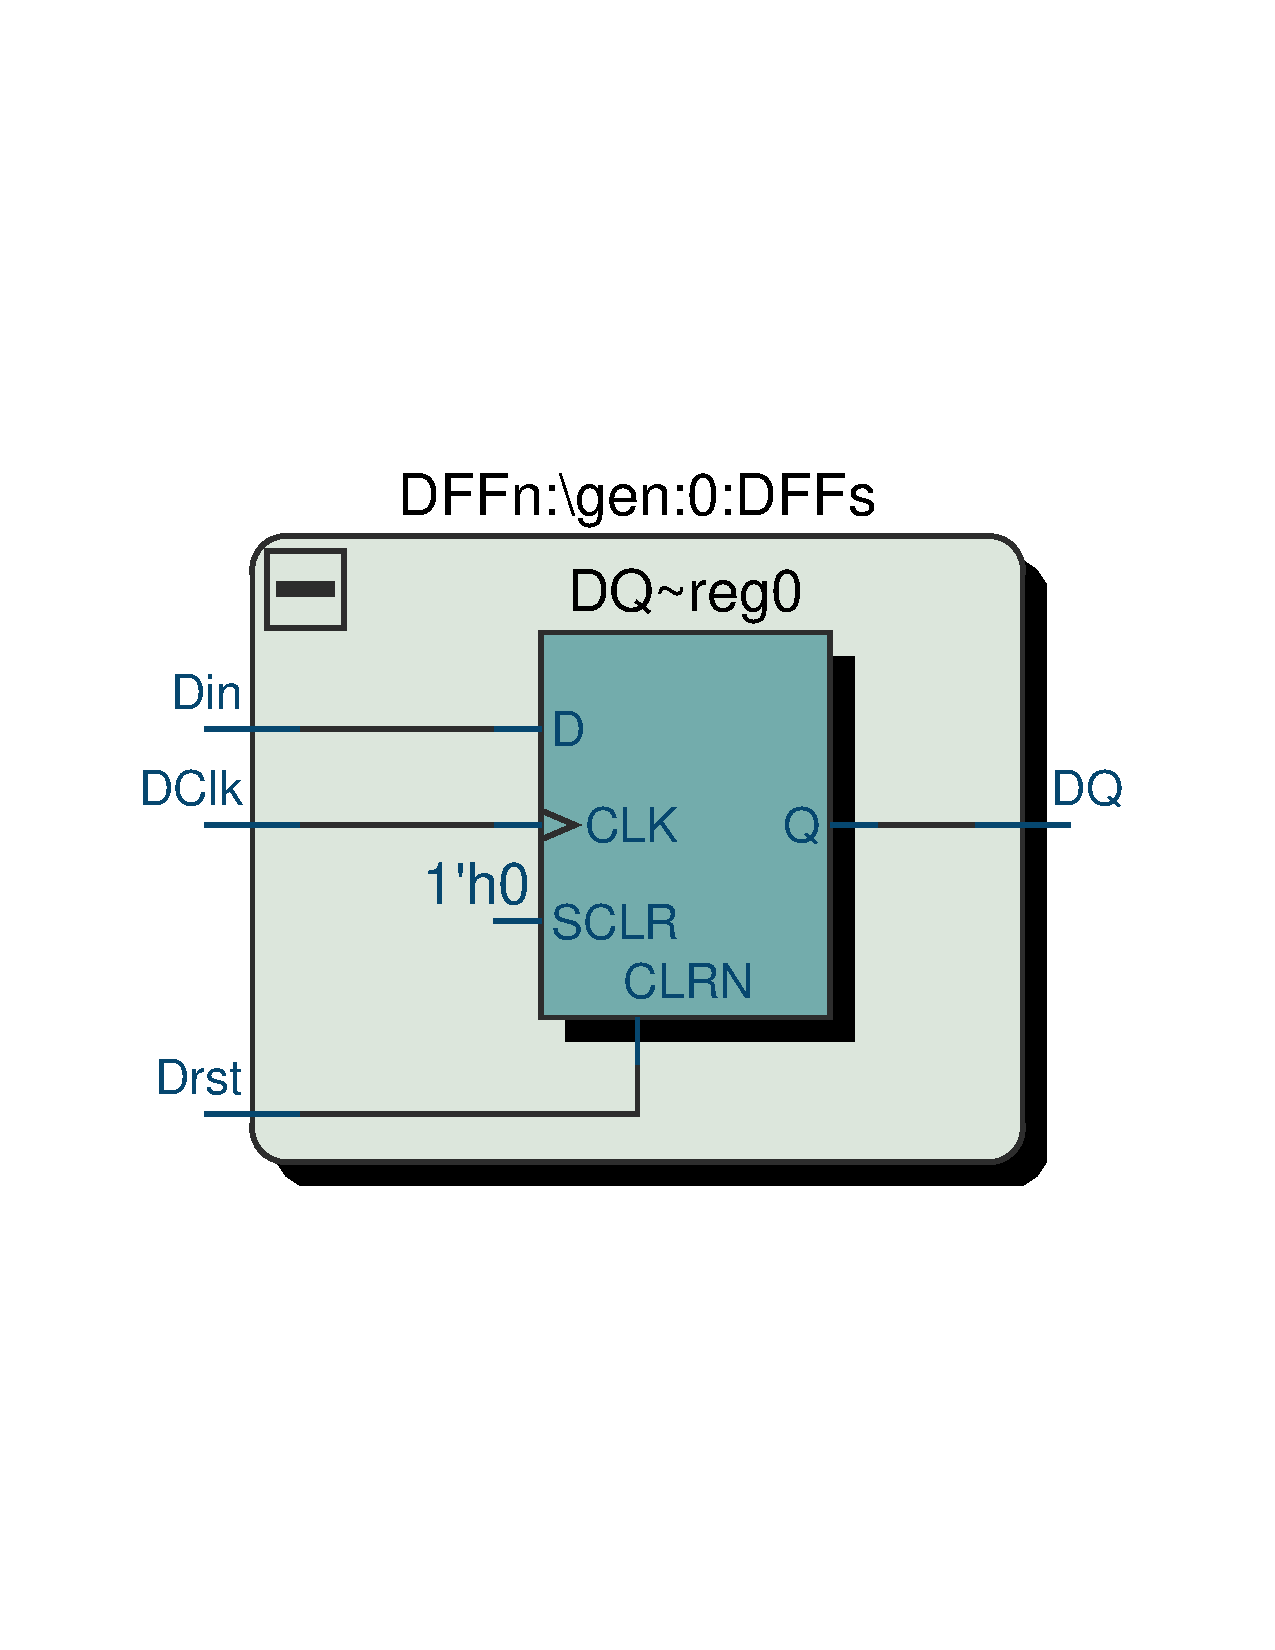
\includegraphics[scale=0.4, clip, trim={2cm 8cm 2cm 9.1cm}]{images/Exc1_DFF_RTL.pdf}
\caption*{D flip-flop}
\end{figure}

\begin{figure}[H]
\centering
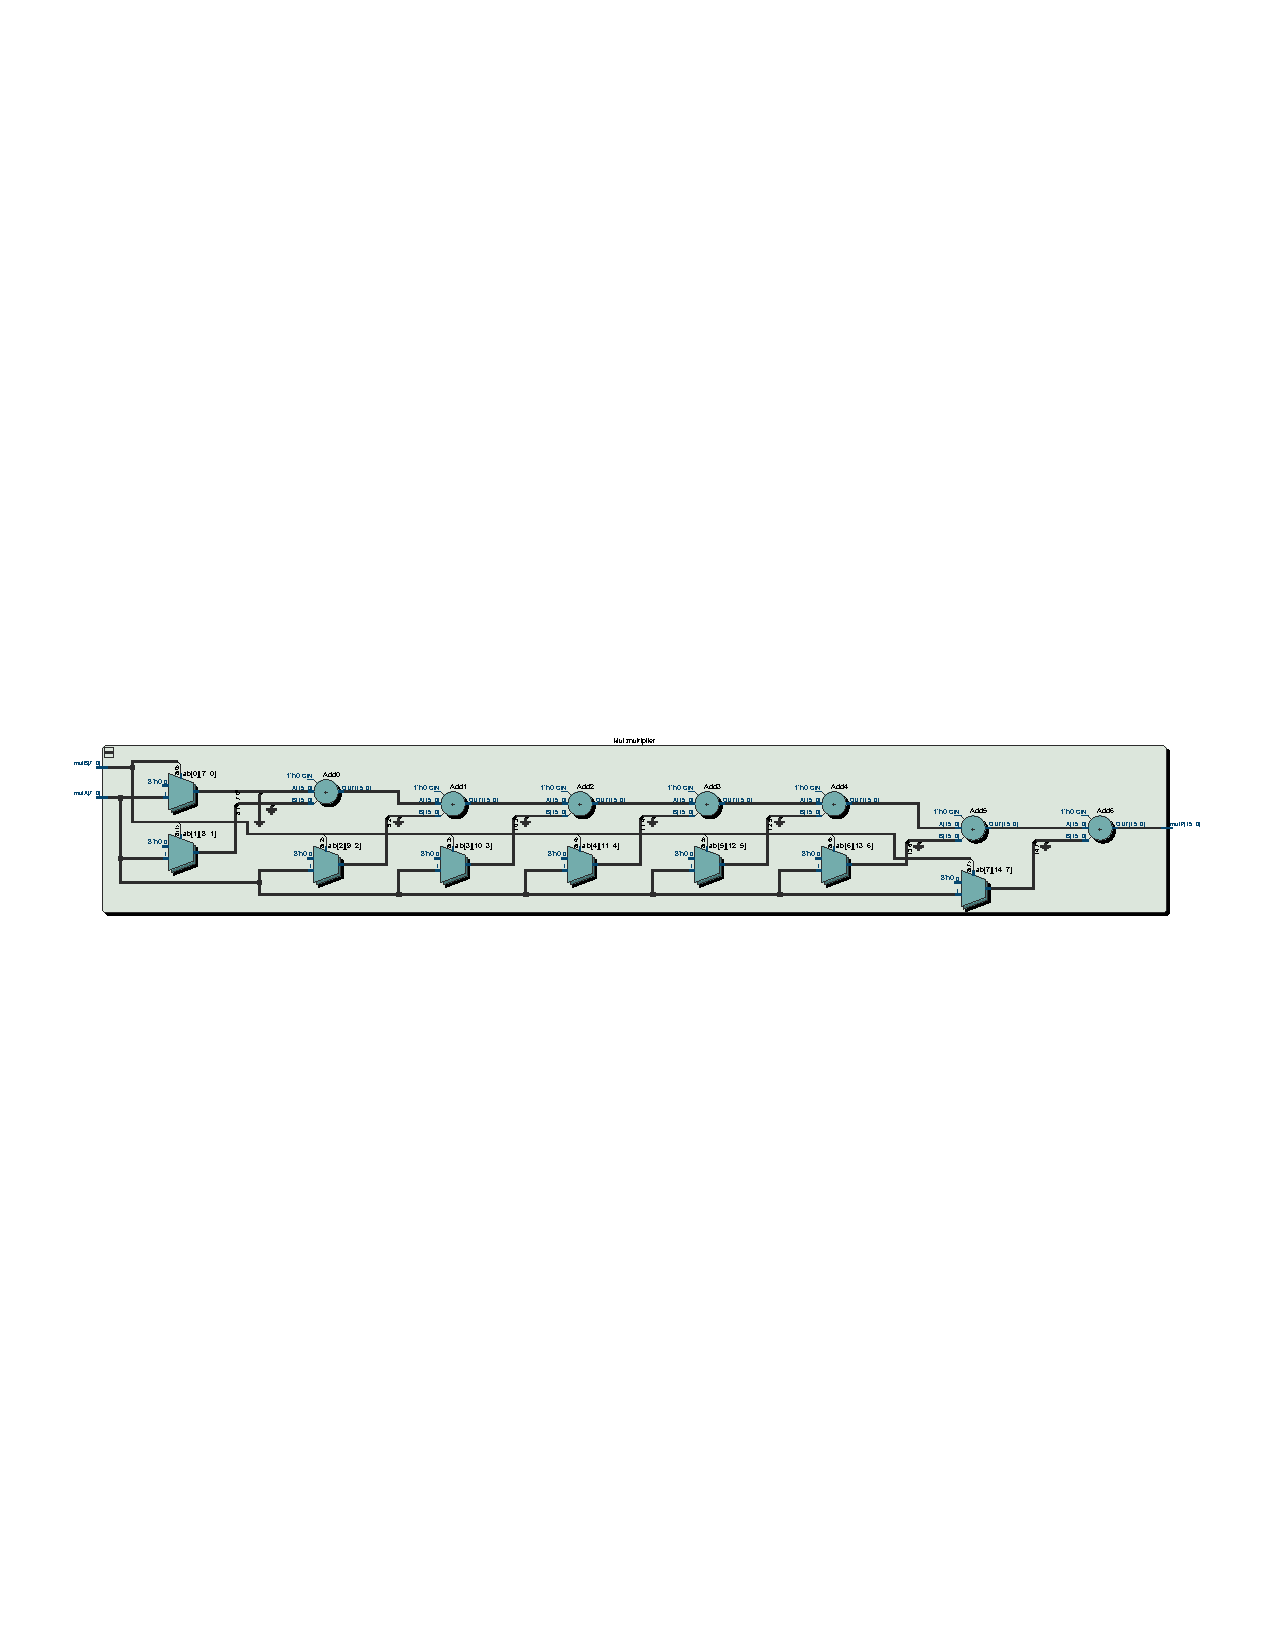
\includegraphics[scale=0.85, clip, trim={0cm 12.3cm 0cm 12.62cm}]{images/Exc3_Mul_RTL.pdf}
\caption*{Multiplier}
\end{figure}

\begin{figure}[H]
\centering
\subfloat[][HEX display decoder]{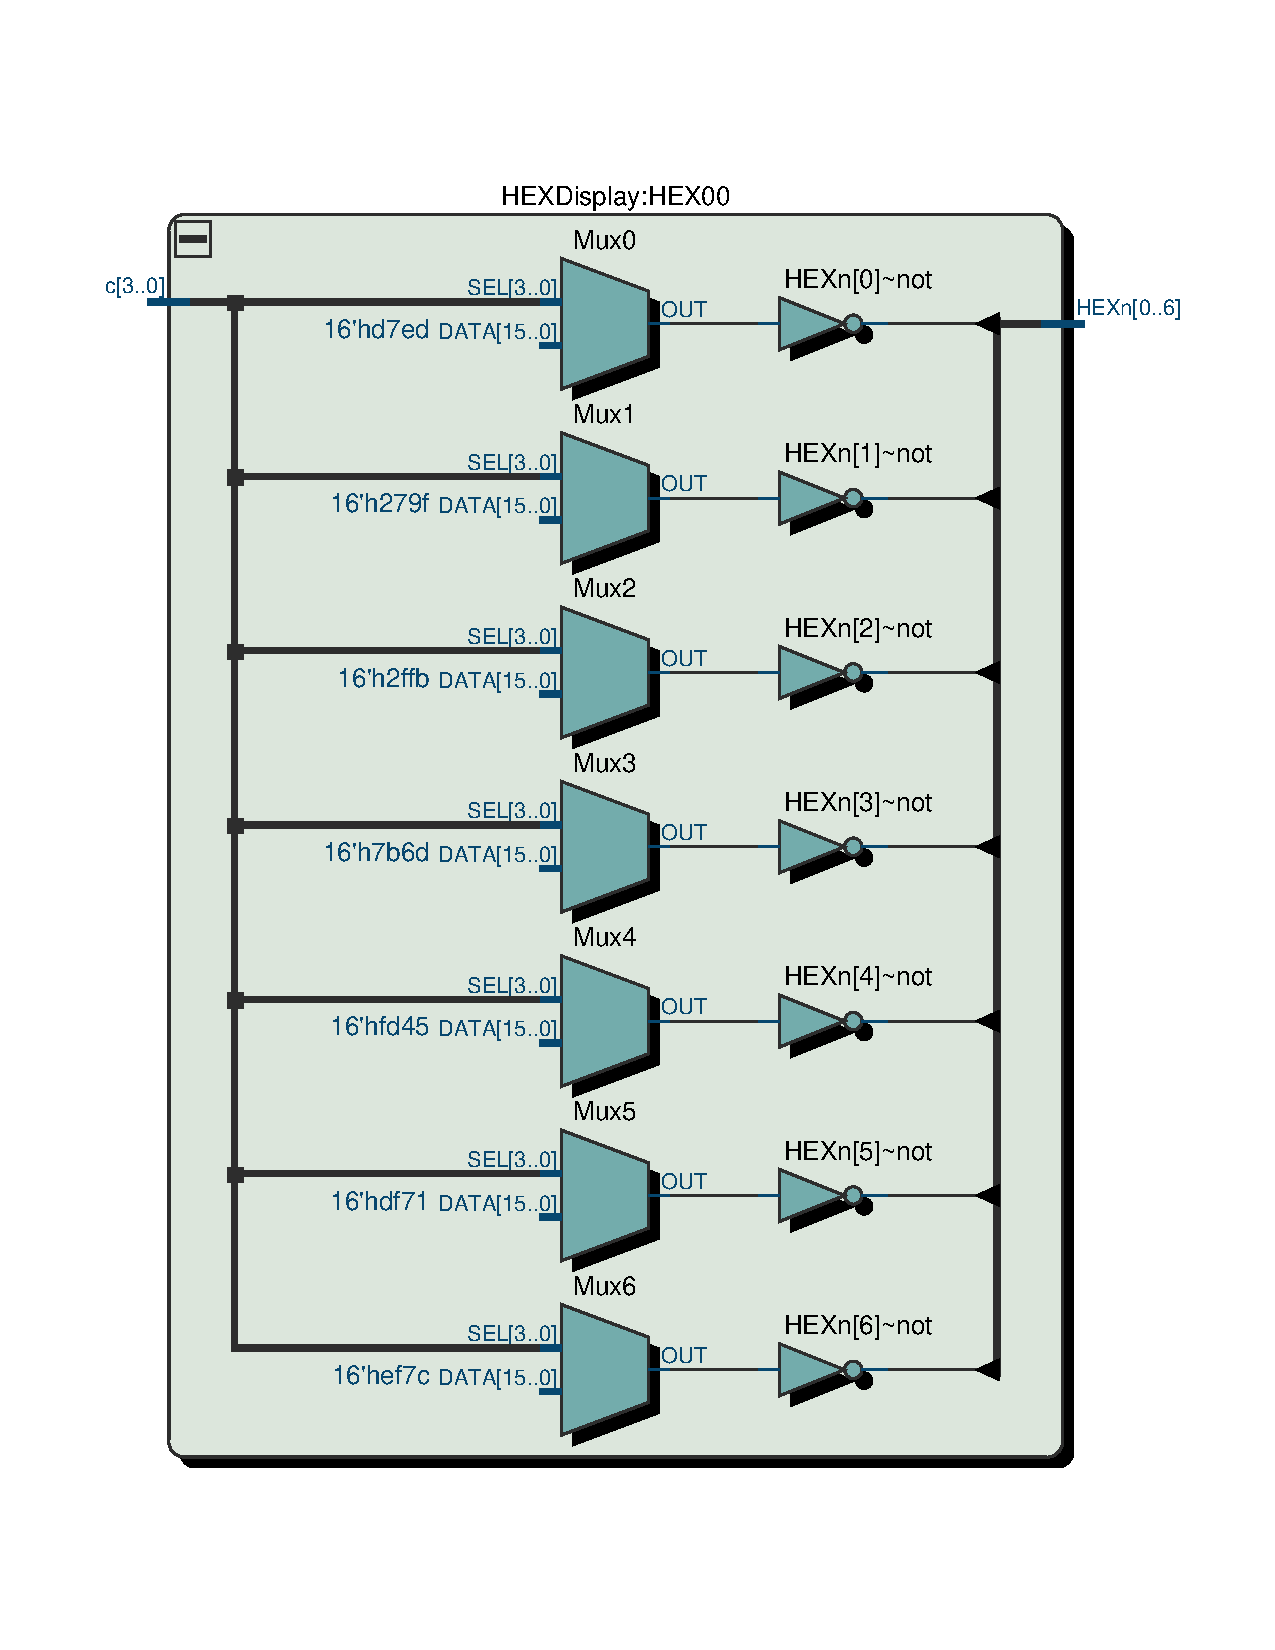
\includegraphics[scale=0.55, clip, trim={2cm 3cm 2cm 3.6cm}]{images/Exc1_HEXDisplay_RTL.pdf}}
\subfloat[][8-bit register]{\includegraphics[scale=0.45, clip, trim={3cm 1cm 3cm 1.6cm}]{images/Exc1_EightBitReg_RTL.pdf}}
\end{figure}


\begin{figure}[H]
\centering
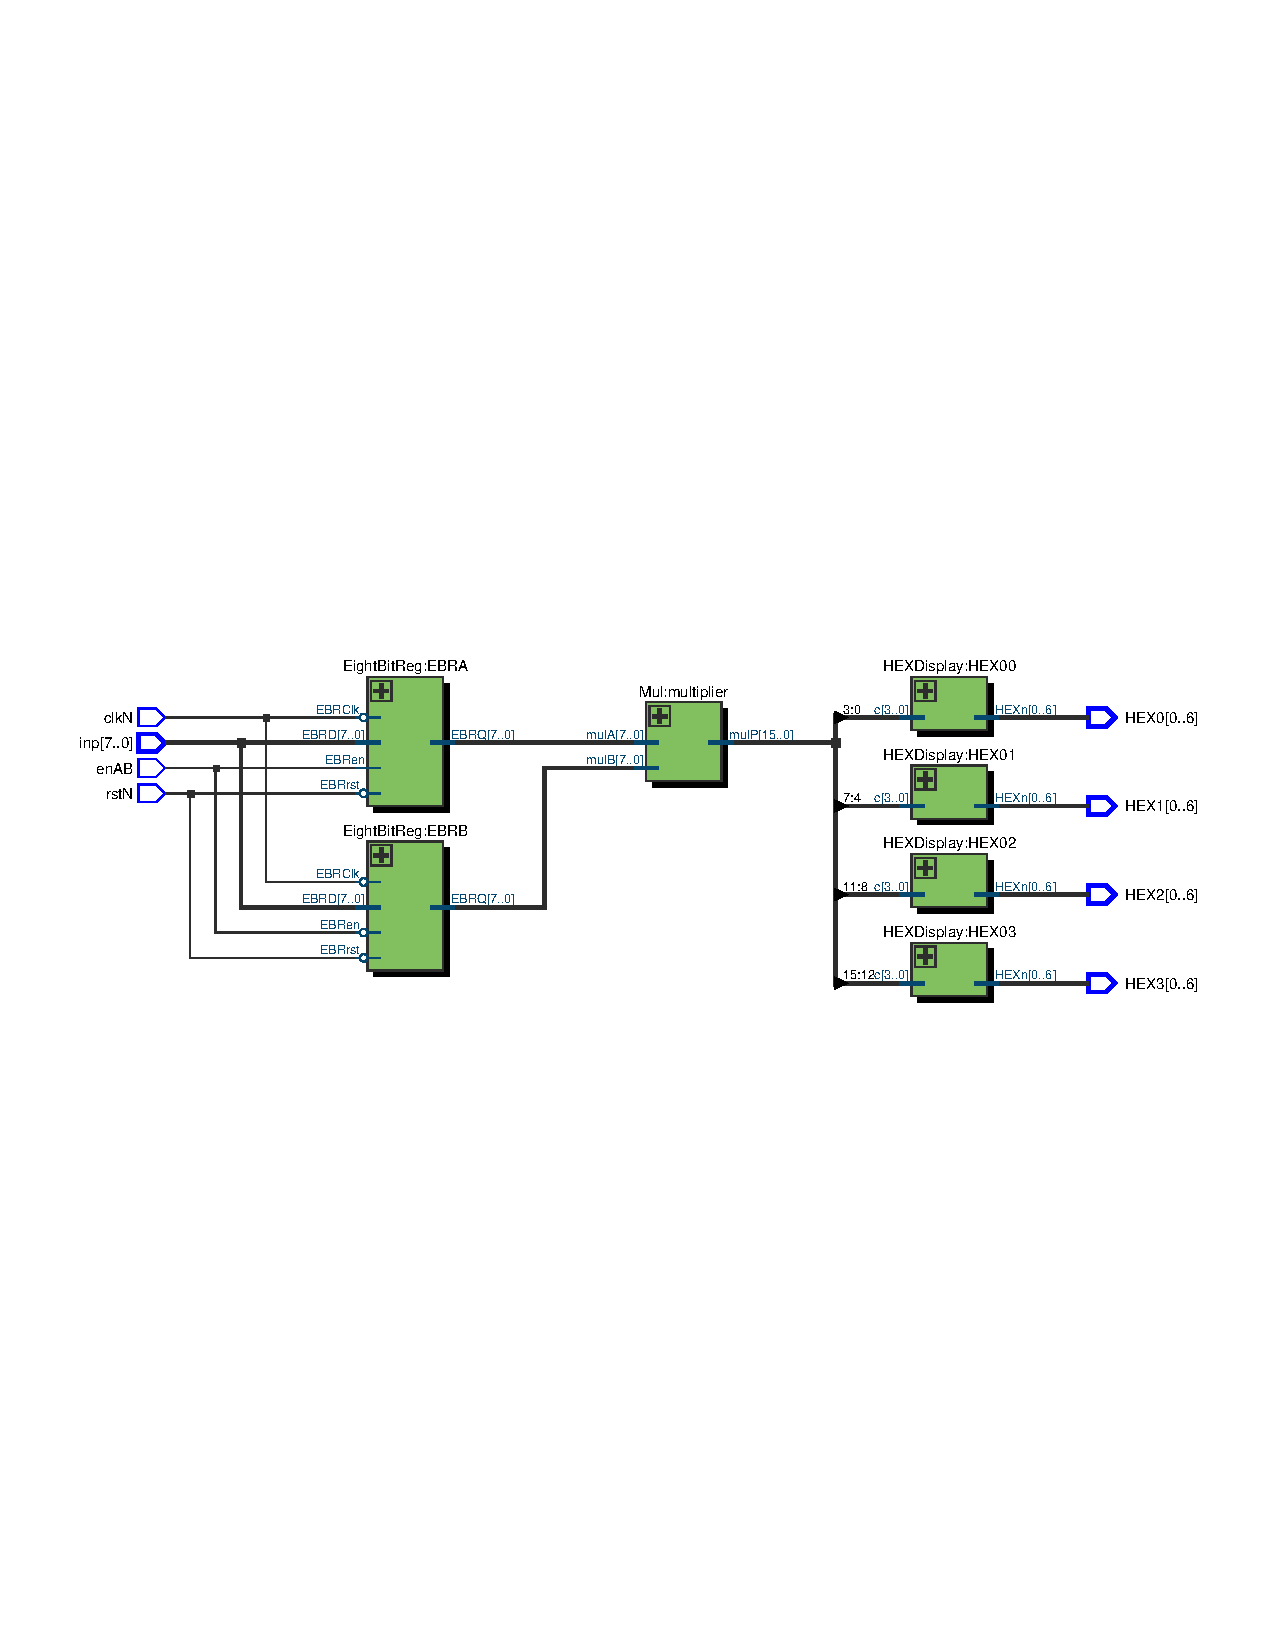
\includegraphics[scale=0.85, clip, trim={0cm 11cm 0cm 11cm}]{images/Exc3_RTL.pdf}
\caption*{Top level}
\end{figure}

\section{Known how to program ALU circuit with registered inputs and outputs.}
I changed the circuit a bit in order to work on a limited-input devices such as DE10.

First, change SW[7:0] to the desired number $A$. Push KEY1 (clk) to store the value into $A$ register.

Then, change SW[7:0] to the desired number $B$. Push KEY1 (clk) while holding KEY2 to store the value into $B$ register.

Or, you can input $B$ first, then $A$ later.

Lastly, change SW[9:8] to 00, 01, 10 or 11 for $A+B$, $A-B$, $B-A$ or $A\times B$, respectively. The result will show up on HEX[3:0].

An example is shown in the waveform section.

\subsection{Code}
\subsubsection{DFFn.vhd}
\begin{minted}{vhdl}
LIBRARY ieee;
USE ieee.std_logic_1164.ALL;
ENTITY DFFn IS
	PORT (
		Din, DClk, Drst : IN STD_LOGIC;
		DQ : OUT STD_LOGIC);
END DFFn;
ARCHITECTURE Behavior OF DFFn IS
BEGIN
	PROCESS (Drst, DClk)
	BEGIN
		IF rising_edge(DClk) THEN
			DQ <= Din;
		END IF;
		IF Drst = '1' THEN
			DQ <= '0';
		END IF;
	END PROCESS;
END Behavior;
\end{minted}

\subsubsection{EightBitReg.vhd}
\begin{minted}{vhdl}
LIBRARY ieee;
USE ieee.std_logic_1164.ALL;
USE ieee.numeric_std.ALL;

ENTITY EightBitReg IS
	PORT (
		EBRClk, EBRrst : IN STD_LOGIC;
		EBRD : IN STD_LOGIC_VECTOR(7 DOWNTO 0);
		EBRQ : OUT STD_LOGIC_VECTOR(7 DOWNTO 0)
	);
END EightBitReg;

ARCHITECTURE arch OF EightBitReg IS
	COMPONENT DFFn IS
		PORT (
			Din, DClk, Drst : IN STD_LOGIC;
			DQ : OUT STD_LOGIC);
	END COMPONENT;
BEGIN
	gen : FOR i IN 7 DOWNTO 0 GENERATE
		DFFs : DFFn PORT MAP(Din => EBRD(i), DClk => EBRClk, Drst => EBRrst, DQ => EBRQ(i));
	END GENERATE;
END ARCHITECTURE;
\end{minted}

\subsubsection{Mul.vhd}
\begin{minted}{vhdl}
LIBRARY ieee;
USE ieee.std_logic_1164.ALL;
USE ieee.std_logic_unsigned.ALL;
USE IEEE.numeric_std.ALL;

ENTITY Mul IS
	PORT (
		mulA, mulB : IN STD_LOGIC_VECTOR(7 DOWNTO 0);
		mulP : OUT STD_LOGIC_VECTOR(15 DOWNTO 0)
	);
END Mul;

ARCHITECTURE arch OF Mul IS
	SIGNAL a_padded, zero : STD_LOGIC_VECTOR(15 DOWNTO 0);
	TYPE ab_t IS ARRAY(0 TO 7) OF STD_LOGIC_VECTOR(15 DOWNTO 0);
	SIGNAL ab : ab_t;
BEGIN

	zero <= "0000000000000000";
	a_padded <= "00000000" & mulA;

	ab(0) <= a_padded WHEN mulB(0) = '1' ELSE
	zero;
	sum : FOR i IN 1 TO 7 GENERATE
		ab(i) <= a_padded(15 - i DOWNTO 0) & zero(i - 1 DOWNTO 0) WHEN mulB(i) = '1' ELSE
		zero;
	END GENERATE;

	mulP <= ab(0) + ab(1) + ab(2) + ab(3) + ab(4) + ab(5) + ab(6) + ab(7);
END ARCHITECTURE;
\end{minted}

\subsubsection{HEXDisplay.vhd}
\begin{minted}{vhdl}
LIBRARY ieee;
USE ieee.std_logic_1164.ALL;

ENTITY HEXDisplay IS
	PORT (
		c : IN STD_LOGIC_VECTOR(3 DOWNTO 0);
		HEXn : OUT STD_LOGIC_VECTOR(0 TO 6)
	);
END HEXDisplay;

ARCHITECTURE behavior OF HEXDisplay IS
	SIGNAL HEX : STD_LOGIC_VECTOR(0 TO 6);
BEGIN
	HEXn <= NOT(HEX);
	WITH c SELECT
		HEX <= "1111110" WHEN "0000",
		"0110000" WHEN "0001",
		"1101101" WHEN "0010",
		"1111001" WHEN "0011",
		"0110011" WHEN "0100",
		"1011011" WHEN "0101",
		"1011111" WHEN "0110",
		"1110000" WHEN "0111",
		"1111111" WHEN "1000",
		"1111011" WHEN "1001",

		"1110111" WHEN "1010",
		"0011111" WHEN "1011",
		"1001110" WHEN "1100",
		"0111101" WHEN "1101",
		"1001111" WHEN "1110",
		"1000111" WHEN "1111",
		"0000000" WHEN OTHERS;
END behavior; -- behavior
\end{minted}

\subsubsection{Exc3.vhd}
\begin{minted}{vhdl}
LIBRARY ieee;
USE ieee.std_logic_1164.ALL;
USE ieee.numeric_std.ALL;

ENTITY Exc4 IS
	PORT (
		inp : IN STD_LOGIC_VECTOR(7 DOWNTO 0);
		HEX3, HEX2, HEX1, HEX0 : OUT STD_LOGIC_VECTOR(0 TO 6);
		enAB, clkN, rstN : IN STD_LOGIC;
		sel : IN STD_LOGIC_VECTOR(1 DOWNTO 0)
	);
END Exc4;

ARCHITECTURE arch OF Exc4 IS
	SIGNAL a, b : STD_LOGIC_VECTOR(7 DOWNTO 0);
	SIGNAL sum, subAB, subBA : STD_LOGIC_VECTOR(15 DOWNTO 0);
	SIGNAL p, result : STD_LOGIC_VECTOR(15 DOWNTO 0);
	SIGNAL clk, rst : STD_LOGIC;

	COMPONENT EightBitReg IS
		PORT (
			EBRClk, EBRrst, EBRen : IN STD_LOGIC;
			EBRD : IN STD_LOGIC_VECTOR(7 DOWNTO 0);
			EBRQ : OUT STD_LOGIC_VECTOR(7 DOWNTO 0)
		);
	END COMPONENT;

	COMPONENT Mul IS
		PORT (
			mulA, mulB : IN STD_LOGIC_VECTOR(7 DOWNTO 0);
			mulP : OUT STD_LOGIC_VECTOR(15 DOWNTO 0)
		);
	END COMPONENT;

	COMPONENT HEXDisplay IS
		PORT (
			c : IN STD_LOGIC_VECTOR(3 DOWNTO 0);
			HEXn : OUT STD_LOGIC_VECTOR(0 TO 6)
		);
	END COMPONENT;
BEGIN
	rst <= NOT(rstN);
	clk <= NOT(clkN);
	EBRA : EightBitReg PORT MAP(
		EBRClk => clk, EBRrst => rst,
		EBRen => NOT(enAB), EBRD => inp, EBRQ => a);
	EBRB : EightBitReg PORT MAP(
		EBRClk => clk, EBRrst => rst,
		EBRen => enAB, EBRD => inp, EBRQ => b);

	multiplier : Mul PORT MAP(mulA => a, mulB => b, mulP => p);
	sum <= STD_LOGIC_VECTOR(unsigned("00000000" & a) + unsigned("00000000" & b));
	subAB <= STD_LOGIC_VECTOR(unsigned("00000000" & a) - unsigned("00000000" & b));
	subBA <= STD_LOGIC_VECTOR(unsigned("00000000" & b) - unsigned("00000000" & a));

	WITH sel SELECT
		result <= p WHEN "11",
		sum WHEN "00",
		subAB WHEN "01",
		subBA WHEN "10";
	HEX03 : HEXDisplay PORT MAP(c => result(15 DOWNTO 12), HEXn => HEX3);
	HEX02 : HEXDisplay PORT MAP(c => result(11 DOWNTO 8), HEXn => HEX2);
	HEX01 : HEXDisplay PORT MAP(c => result(7 DOWNTO 4), HEXn => HEX1);
	HEX00 : HEXDisplay PORT MAP(c => result(3 DOWNTO 0), HEXn => HEX0);
END ARCHITECTURE;
\end{minted}

\subsection{Waveform}
\begin{table}[H]
\centering
\begin{tabular}{cccc|cccccc}
\multirow{2}{*}{$A$} & \multirow{2}{*}{$B$} & \multirow{2}{*}{Select} & \multirow{2}{*}{Operation} & \multirow{2}{*}{$P$} & \multirow{2}{*}{7-segment display} & \multicolumn{4}{c}{HEX output (active low)} \\
                     &                      &                         &                            &                      &                                    & 3         & 2         & 1        & 0        \\ \hline
B9                   & E6                   & 00                      & $A+B$                      & 019F                 & \hex{0}{1}{9}{f}                   & 0000001   & 1001111   & 0000100  & 0111000  \\
                     &                      & 01                      & $A-B$                      & FFD3                 & \hex{f}{f}{d}{3}                   & 0111000   & 0111000   & 1000010  & 0000110  \\
                     &                      & 10                      & $B-A$                      & 002D                 & \hex{0}{0}{2}{d}                   & 0000001   & 0000001   & 0010010  & 1000010  \\
                     &                      & 11                      & $A \times B$               & A636                 & \hex{a}{6}{3}{6}                   & 0001000   & 0100000   & 0000110  & 0100000  \\ \hline
32                   & F2                   & 00                      & $A+B$                      & 0124                 & \hex{0}{1}{2}{4}                   & 0000001   & 1001111   & 0010010  & 1001100  \\
                     &                      & 01                      & $A-B$                      & FF40                 & \hex{f}{f}{4}{0}                   & 0111000   & 0111000   & 1001100  & 0000001  \\
                     &                      & 10                      & $B-A$                      & 00C0                 & \hex{0}{0}{c}{0}                   & 0000001   & 0000001   & 0110001  & 0000001  \\
                     &                      & 11                      & $A \times B$               & 2F44                 & \hex{2}{f}{4}{4}                   & 0010010   & 0111000   & 1001100  & 1001100 
\end{tabular}
\end{table}

\begin{figure}[H]
\centering
\includegraphics[scale=0.4]{images/Exc4_waveform.png}
\end{figure}

\subsection{Result of RTL viewer}


\begin{figure}[H]
\centering
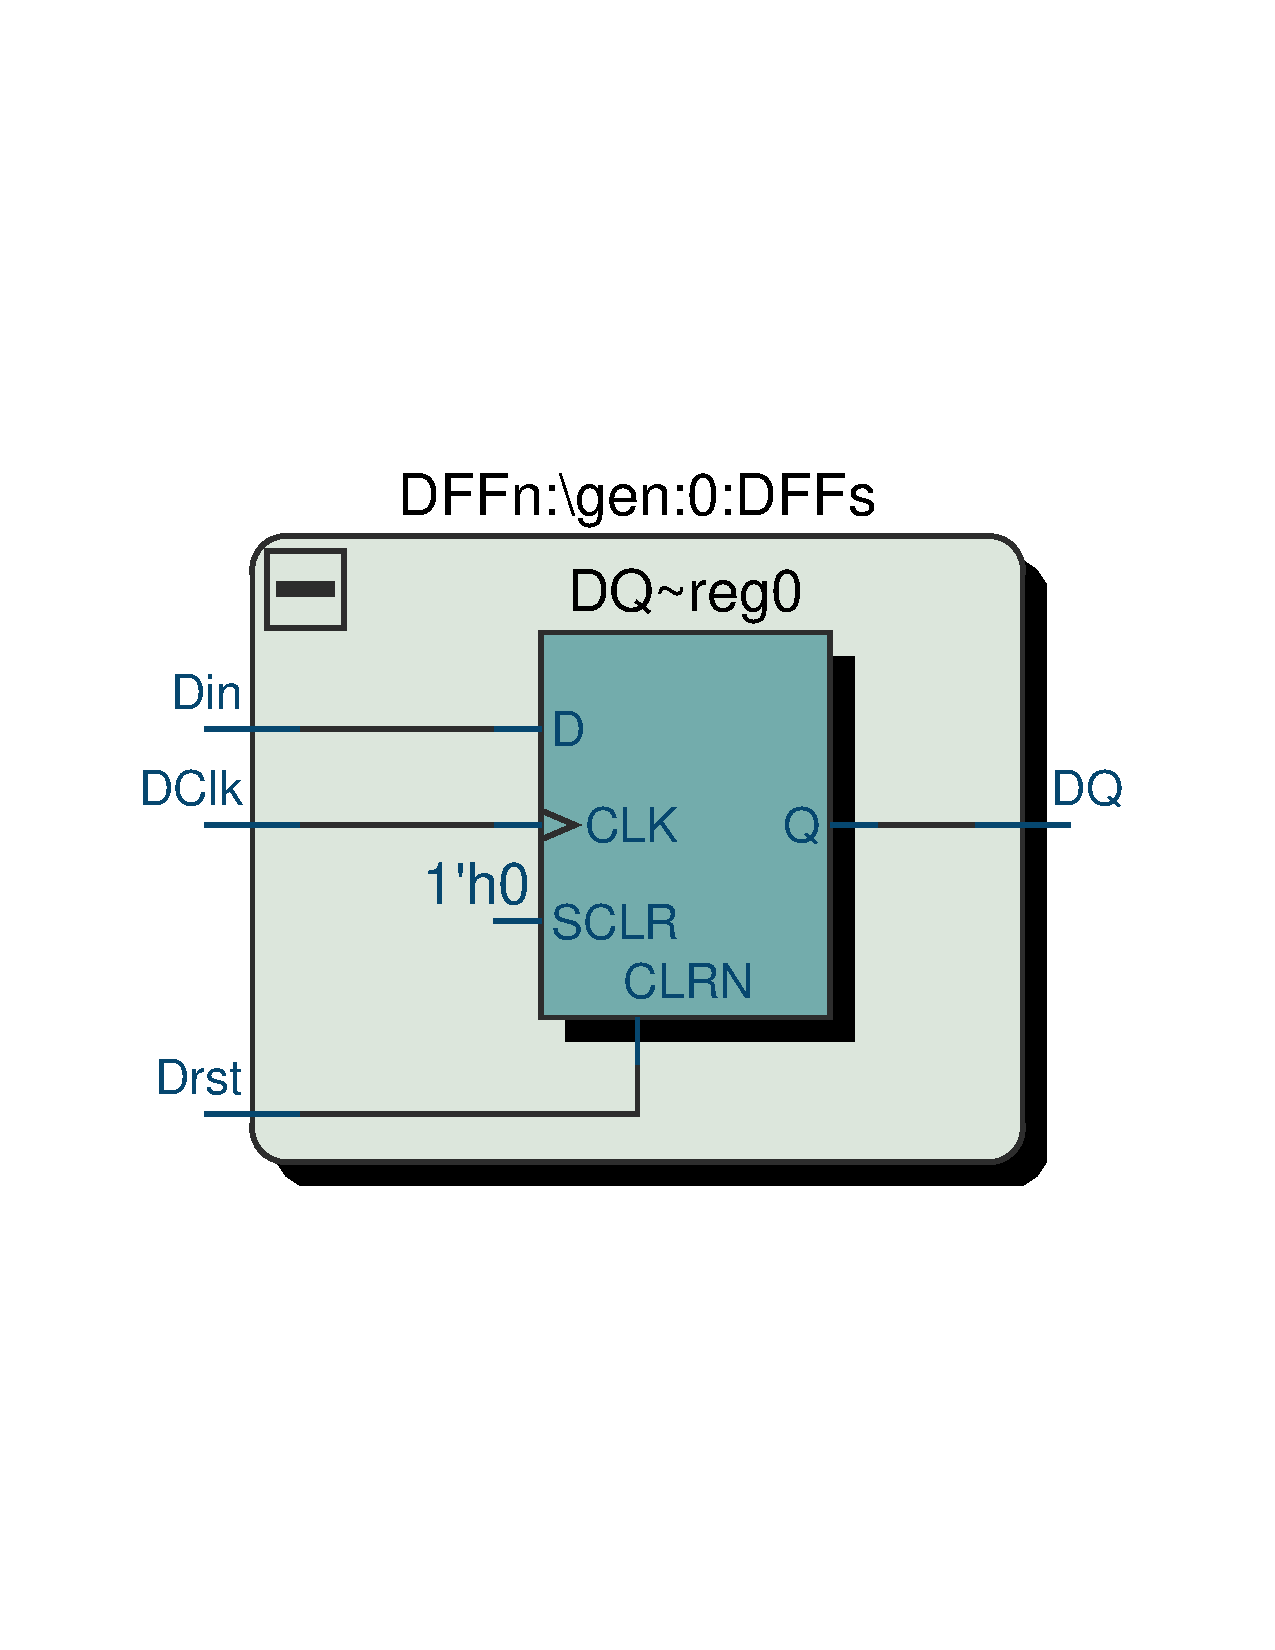
\includegraphics[scale=0.4, clip, trim={2cm 8cm 2cm 9.1cm}]{images/Exc1_DFF_RTL.pdf}
\caption*{D flip-flop}
\end{figure}

\begin{figure}[H]
\centering
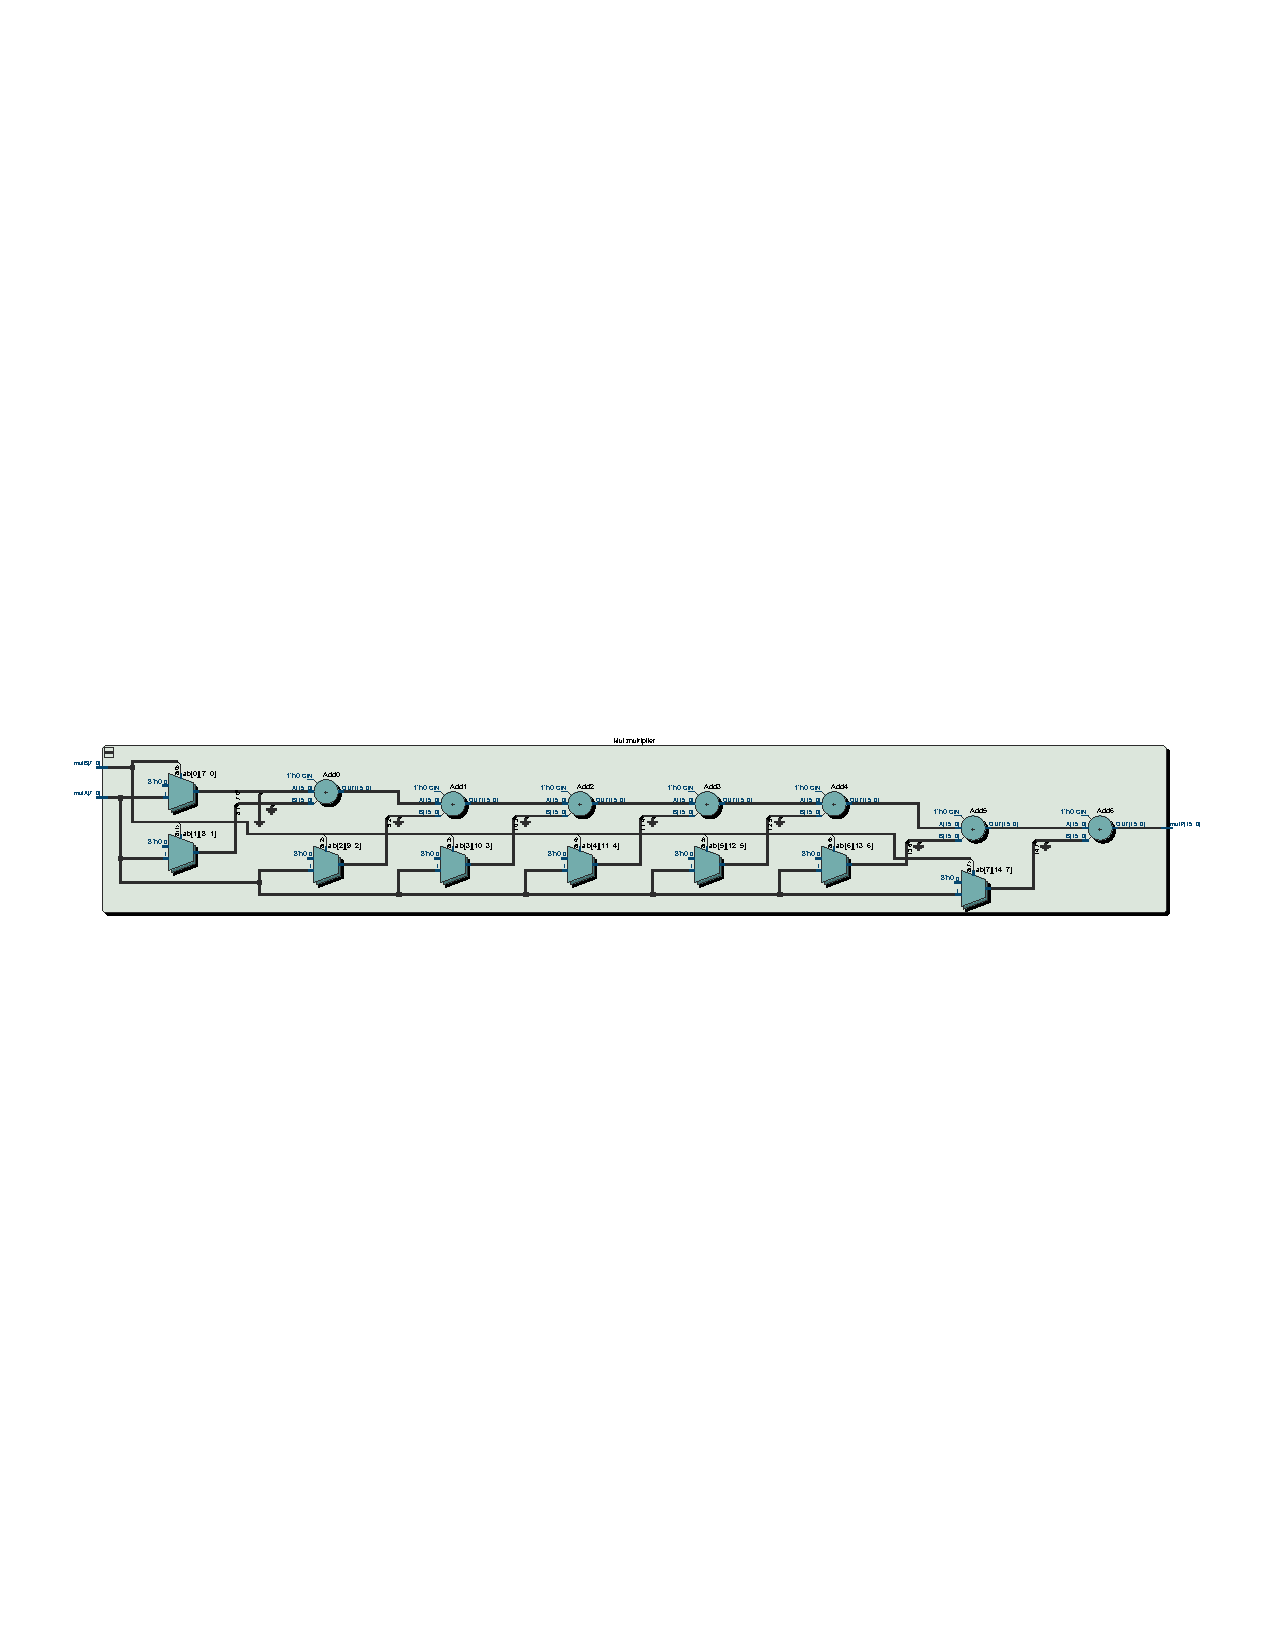
\includegraphics[scale=0.85, clip, trim={0cm 12.3cm 0cm 12.62cm}]{images/Exc3_Mul_RTL.pdf}
\caption*{Multiplier}
\end{figure}

\begin{figure}[H]
\centering
\subfloat[][HEX display decoder]{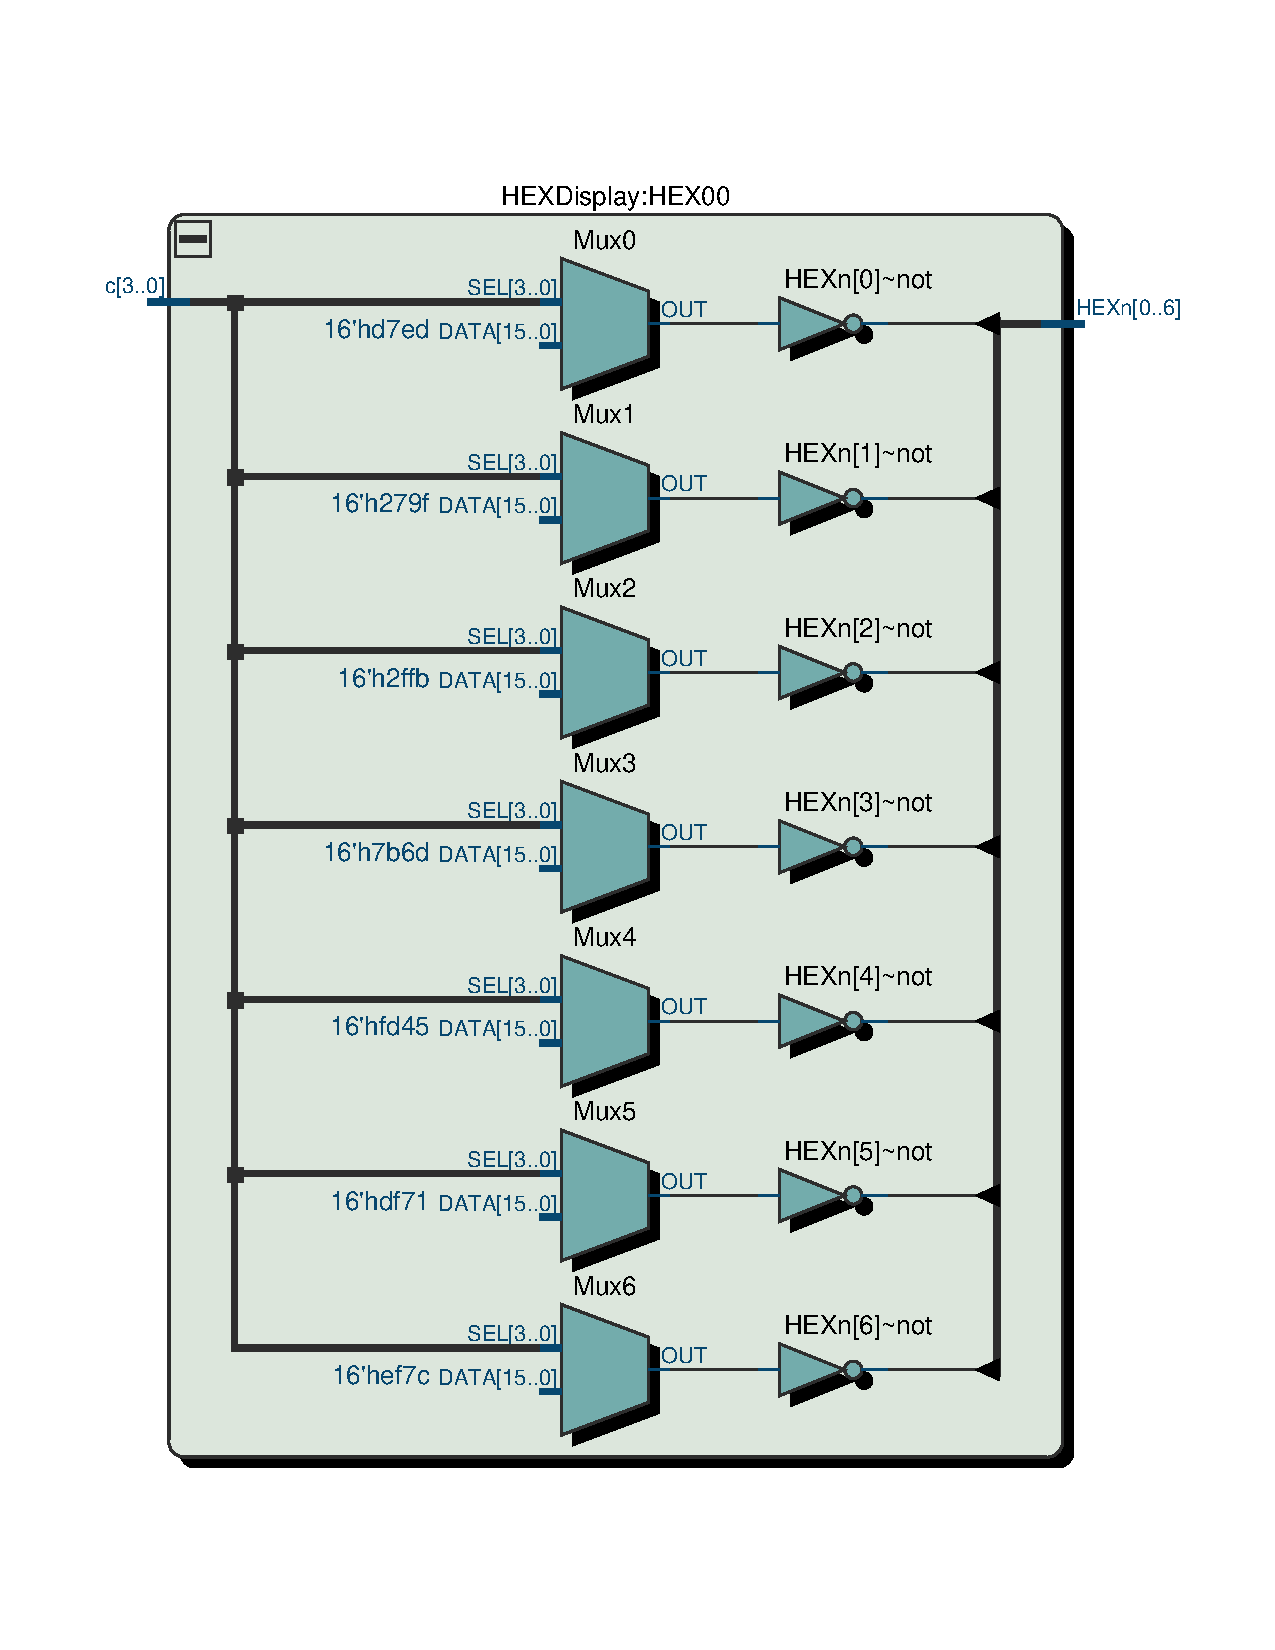
\includegraphics[scale=0.55, clip, trim={2cm 3cm 2cm 3.6cm}]{images/Exc1_HEXDisplay_RTL.pdf}}
\subfloat[][8-bit register]{\includegraphics[scale=0.45, clip, trim={3cm 1cm 3cm 1.6cm}]{images/Exc1_EightBitReg_RTL.pdf}}
\end{figure}


\begin{figure}[H]
\centering
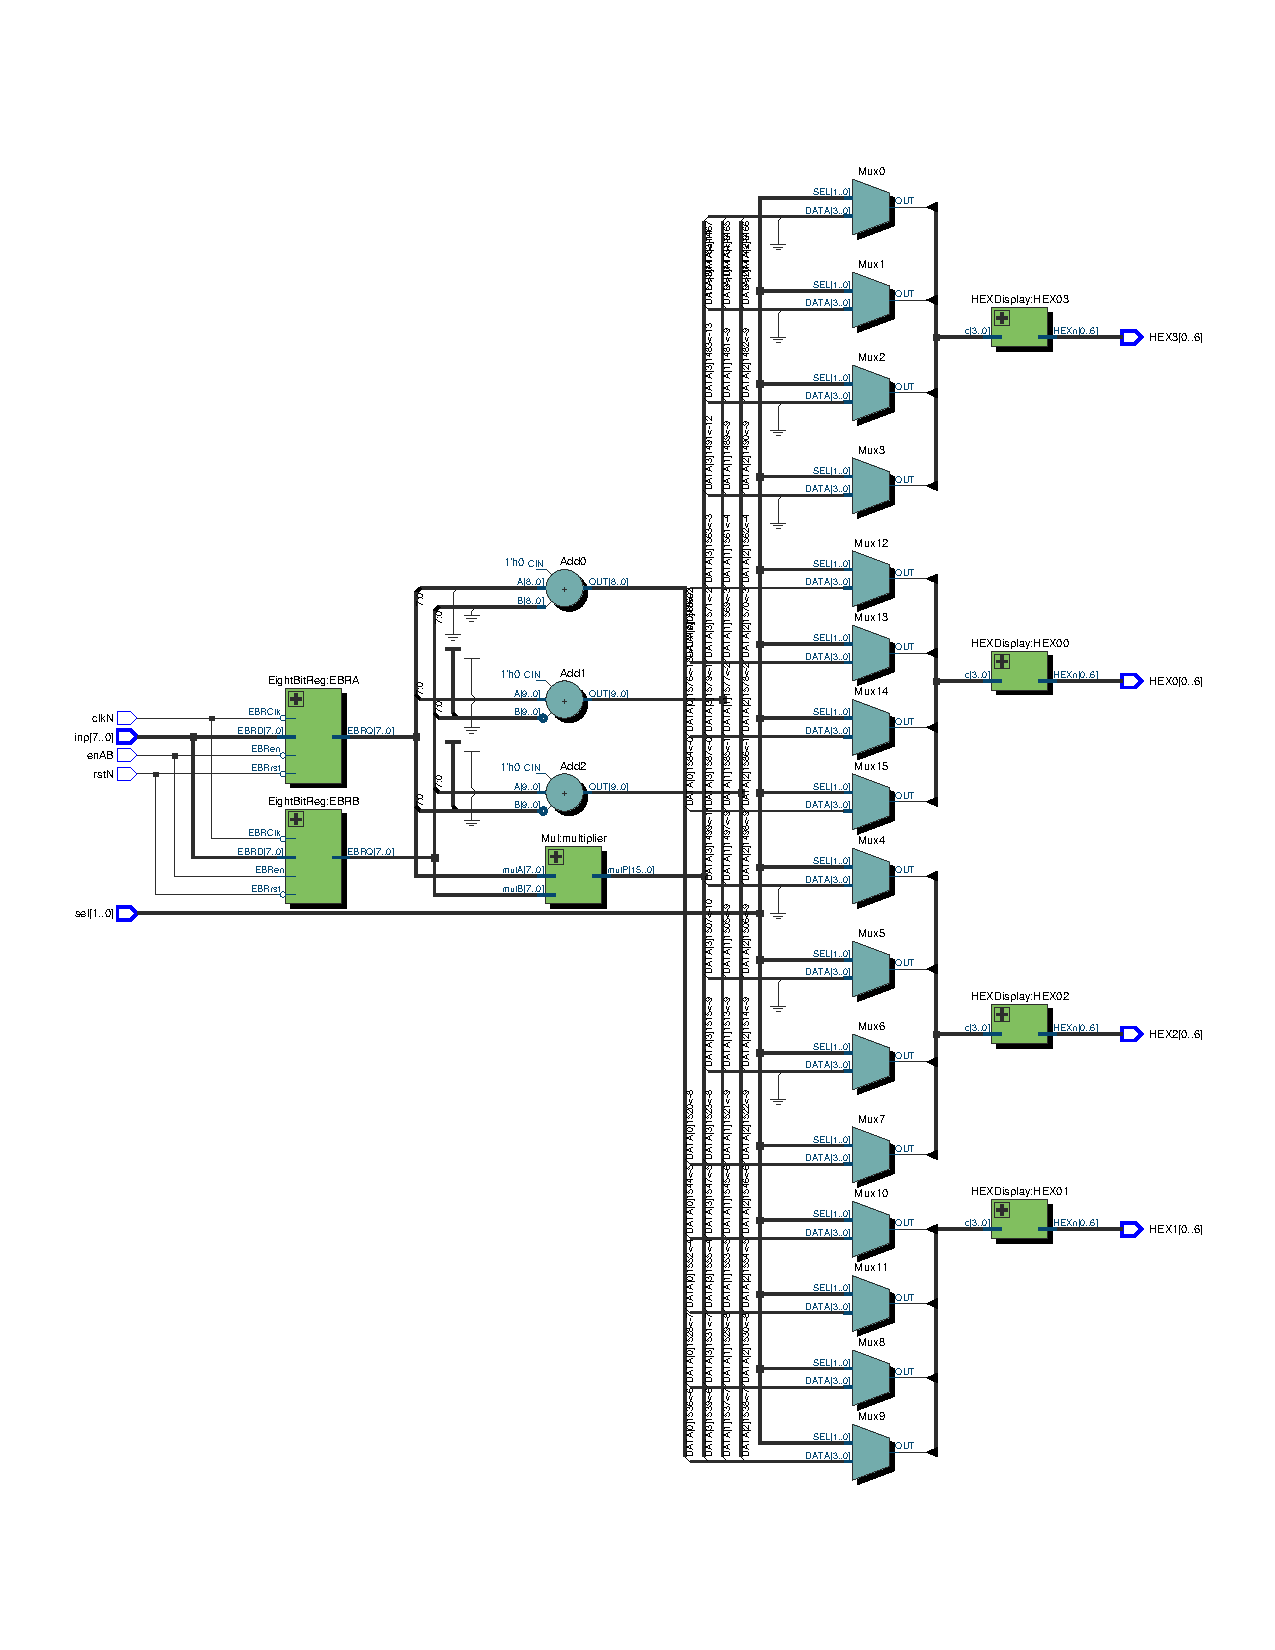
\includegraphics[scale=0.85, clip, trim={0cm 2cm 0cm 2cm}]{images/Exc4_RTL.pdf}
\caption*{Top level}
\end{figure}

\end{document}